\chapter{Results}
{\samenvatting todo}
\section{Person specific}
At first research was done in a person specific setting. This means that that algorithm was trained on several samples from a single person, before it was tested on the same person.
This section will go over the results.

\npar

The first step was to transform the continuous valence and arousal values to classes. This was done by performing a simple binary classification. Given that the dimension range from 1 to 9, all labels with a valence or arousal below 5 were reported as low valence or arousal respectively. The remaining valence or arousal were placed in the high valence or arousal respectively.

\subsection{Used approach}

This thesis compares the aforementioned features and the aforementioned feature selection methods. For this a two stepped algorithm, inspired by the advanced random forest method, explained in Section \ref{rfmethod}, was used. In short, the first step is to rank all the features and only take the top X of the features. This threshold is applied to limit computation times and throw out features that have very low importance. The next step is to iteratively build a model by selecting features out of the remaining feature set. This approach is depicted in Figure \ref{flow}.

\mijnfiguur{width=0.9\textwidth}{flow}{The used approach of this thesis.}

As you can see in Figure \ref{flow}, the approach starts by separating a test set to evaluate the final performance of the algorithm. This test set contained 10 of the 40 samples. Next, the aforementioned feature selection methods are applied to the train set. A top $X$ of the features is then kept.

\npar

In the next step different models are build. This is done iteratively by starting with an empty feature set. In the add step, a feature is added to this set and the cross validation error is determined. Cross validation is a technique that separates the data in N folds, as shown in Figure \ref{CVscheme}. Next the algorithm is trained on N-1 blocks and tested on the remaining blocks. This is done N times and the average of the performance is then reported as cross validation error. 

%CV fig
\mijnfiguur{width=0.55\textwidth}{CVscheme}{Cross validation}

The advantage of using a cross validation scheme is that it gives a pretty good estimation of the generalisation of the algorithm, while still using all train data. This step is important because it ensure that the chosen features have good generalisation properties. Good feature should perform well on unseen samples. Note that the test set, displayed in red is not used during cross validation. The test set is kept completely separate to ensure that a fair estimate of the generalisation is achieved.

\npar

Next the average of the cross validation errors and the standard deviation is calculated. The average cross validation minus the standard deviation is b
then compared to the previous best performance. If the performance is better, the feature is kept in the feature set. If the performance is not better, the feature is neglected. The standard deviation is included to increase the stability of the algorithm. By making sure that the new model performs better in a statistical way, one can avoid that small differences in averages lead to a different model.

\npar

In the final step the performance of the test set is determined by the accuracy metric. Accuracy is chosen as metric, because this metric gives a clear and intuitive measurement of performance.

\npar

%params
The first parameter of this flow is the threshold parameter, indicated in the figure as $X$. This threshold cancels features with low importance, by simply taking the best $X$ features from the feature ranking. Assigning a high value to the threshold will increase calculation times as more features are available for the building phase. The performance of the model, will not be better, since a lot of the additional features will have low importance values. Setting a low threshold is also not good, as this might cancel out important features. 

\npar

In this work, the parameter was fixed to 30 for all feature selection methods for the following reasons. First, considering that there are 30 samples in the feature set, having 30 features is already more than enough. Note that a well-known rule of thumb is to have at least 10 times more samples than features\citep{rot1,rot2}\footnote{Note that this is just a rule of thumb, and therefore not proven theoretically. In practice however, it turns out to work quite well.}. Second, looking at the features that were selected during training, one can see that usually around 5-7 features remain. The last selected feature usually has a rank around 20, meaning that the last 10 available features in the building phase are rarely used.

\npar
 %TODO weg ?
A second parameter of this model is a model to estimate the performance. For this, two different models were compared. The first model is an SVM with a radial basis functions kernel. This model was chose because it has proven itself in multiple emotion recognition studies. Additionally, SVM are capable to handle small dataset, which gives this method an advantage in this experiment. The next model is a random forest with 2000 estimators. This model was mainly chosen, because feature selection with random forest deliver good results, according to literature\citep{rfPaper}. Using the same algorithm in both feature selection and building phase, means that the algorithm can select its own features. In other words features that work well for the specific algorithm are more likely to be chosen as this is done by the same algorithm.

\clearpage

\subsection{Performance}

When looking at the accuracies of the different feature selection models in combination with the SVM, it becomes quickly clear that the results are statistically equivalent. 

The corresponding feature selection method for each bar in Figure \ref{accComp_arousalSVM} and Figure \ref{accComp_valenceSVM} are shown in Table \ref{accCompLbl} below.

\begin{table}[H]
\centering
\begin{tabular}{ll|ll}
\textbf{Number} & \textbf{Feature selection method} & \textbf{Number} & \textbf{Feature selection method} \\
\textbf{0}      & Pearson                           & \textbf{6}      & LDA                      \\
\textbf{1}      & Mutual information                & \textbf{7}      & Lasso regression         \\
\textbf{2}      & Distance correlation              & \textbf{8}      & Ridge regression         \\
\textbf{3}      & ANOVA                             & \textbf{9}      & Random forests           \\
\textbf{4}      & Linear regression                 & \textbf{10}     & PCA                      \\
\textbf{5}      & SVM                      &        &                         
\end{tabular}
\caption{The different feature selection methods and their labels\label{accCompLbl}.}
\end{table}

\mijnfiguur{width=1.\textwidth}{accComp_arousalSVM}{Comparison of different feature selection methods for arousal recognition. The blue bars correspond to filter selection methods. Red bars correspond to wrapper methods and green bars are used for the embedded methods.}

\mijnfiguur{width=1.\textwidth}{accComp_valenceSVM}{Comparison of different feature selection methods for valence recognition. The blue bars correspond to filter selection methods. Red bars correspond to wrapper methods and green bars are used for the embedded methods.}

From a statistical point of view, the performance of these methods is equivalent. However, some differences can be observed when looking at the prediction probabilities. The current model is a classification model, meaning that it divides the valence and arousal into two classes: high and low. The classes are determined by a binary separation. Both valence and arousal range between 1 and 9, so every value between 5 is regarded as a low valence/ arousal. All values above 5 are regarded as high valence/arousal.

\npar

It might be interesting to look at the prediction probability a model gives to its output and the distance of the arousal/valence level to this separation boundary. It is expected that a samples with a valence rating of 9 should be easier to predict that one with a valence rating of 5 or 6. This should be reflected in the prediction probability, i.e. a model should be more certain of extreme valence/ arousal values that lie further away from the separation boundary.

\npar

To investigate this, the Pearson correlation coefficient R is plotted for the model build with the corresponding feature selection methods. The Pearson correlations for arousal are depicted in Figure \ref{arousal_corrs}. The legend can be found in Table \ref{corrsCompLbl}. It is clear that overall the correlations are quite low. In case of ridge regression, the correlation is even negative, meaning that the model is more certain of examples that lie closer to the separation boundary, which is undesired. The correlation for random forest is the highest, followed by linear regression. Note that linear regression might not be the best method as it is known to be unstable. Small changes in the input might lead to different importance values, as discussed in Section \ref{LRBad}.

\begin{table}[H]
\centering
\begin{tabular}{ll|ll}
\textbf{Number} & \textbf{Feature selection method} & \textbf{Number} & \textbf{Feature selection method} \\
\textbf{0}      & Pearson                           & \textbf{6}      & LDA                      \\
\textbf{1}      & Mutual information                & \textbf{7}      & Lasso regression         \\
\textbf{2}      & Distance correlation              & \textbf{8}      & Ridge regression         \\
\textbf{3}      & ANOVA                             & \textbf{9}      & Random forests           \\
\textbf{4}      & Linear regression                 & \textbf{10}     & PCA                      \\
\textbf{5}      & SVM                      &        &                         
\end{tabular}
\caption{The different feature selection methods and their labels\label{corrsCompLbl}.}
\end{table}

\mijnfiguur{width=1.\textwidth}{arousal_corrs}{The pearson correlations of the model's prediction probability versus the distance between the subject's level of arousal and the separation boundary.}

The Pearson correlation coefficients for the valence classification are depicted in Figure \ref{valence_corrs}. The legend can be found in Table \ref{corrsCompLbl}. Again the correlation for the random forest is highest, followed by the distance correlation.

\mijnfiguur{width=1.\textwidth}{valence_corrs}{The pearson correlations of the model's prediction probability versus the distance between the subject's level of valence and the separation boundary.}

Even though one cannot statistically prove that the random forest is the best method in means of performance and the aforementioned certainty correlation, these results are quite positive for random forest. 

\subsection{Selected features}

To compare which features where chosen, the feature set was divided into 9 categories:
\begin{enumerate}
\item \textbf{Power features:} PSD and FE features of a single channel
\item \textbf{Asymmetry features:} DASM, RASM, DCAU and RCAU features that represent a the (a)symmetry between two channels.
\item \textbf{Fractions:} Alpha/beta and fractions of different power ratios of a channels.

\item \textbf{Heart rate:} the statistical values of the heart rate.
\item \textbf{Galvanic skin response:} the statistical values of the GSR.
\item \textbf{Respiration:} the statistical values of the respiration.
\item \textbf{Bloop pressure:} the statistical values of the plethysmograph.
\item \textbf{Skin temp:} the statistical values of the skin temperature.
\end{enumerate} 

The results for arousal are depicted in Figure \ref{arousalpies}, the legend is shown in Figure \ref{arousalpieslegend}. In these plots, a pie chart is shown that gives the distribution all the selected features for all persons combined. When looking at the different selected features for the different feature seleciton methods, it becomes clear that the most valuable features are the asymmetry features combined with the power features.

\npar

One can easily see that the amount of asymmetry features is always the highest, except in case of linear, mutual information and lasso regression. This can be explained by the fact that these methods are not very advanced. Additionally, lasso regression is very prone to noise, as explained earlier in Section \ref{lassoregression}. 

\npar

For arousal one can thus conclude that the different feature selection methods agree mostly on what set of feature categories is relevant. The most import features are the asymmetry features, followed by the power features. The non-EEG features are rarely chose and do not seem to be of importance here. It is also important to note that the fractions of frequency bands is not as important as previously thought. Literature suggested that the fractions of the alpha versus the beta frequency band would give an indication for the arousal of a subject. The main argument for this was the fact that arousal measures how active a person is feeling. A large fraction of alpha and beta power means that the brain is in a relaxed state or in an active and focussed state respectively. Looking at these fractions was therefore supposed to give insight in the arousal level of a subject. These results indicate that the asymmetry and power features are more relevant.

\npar

The results for valence are depicted in Figure \ref{valencepies} and the corresponding legend in Figure \ref{valencepieslegend}. The selected features are similar to the selected features for arousal recognition. The most valuable features are again the asymmetry and power features. These results were expected, most of the emotion recognition studies agree that the asymmetry features give insight in the valence level of a subject. Again we see that some less advanced methods value the power features more.

\clearpage
\begin{figure}[!tbp]
  \centering
  \caption{Selection features for arousal classification.\label{arousalpies}}
  \begin{subfigure}[b]{0.3\textwidth}
    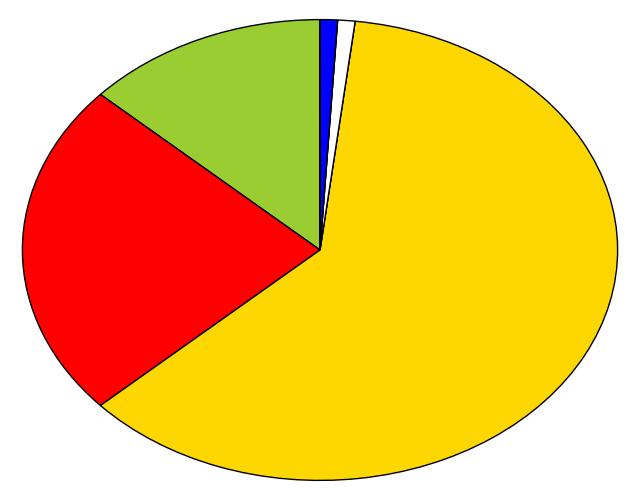
\includegraphics[width=\textwidth]{arousalALLpearsonR}
    \caption{Pearson correlation}
  \end{subfigure}
  \hfill
  \begin{subfigure}[b]{0.3\textwidth}
    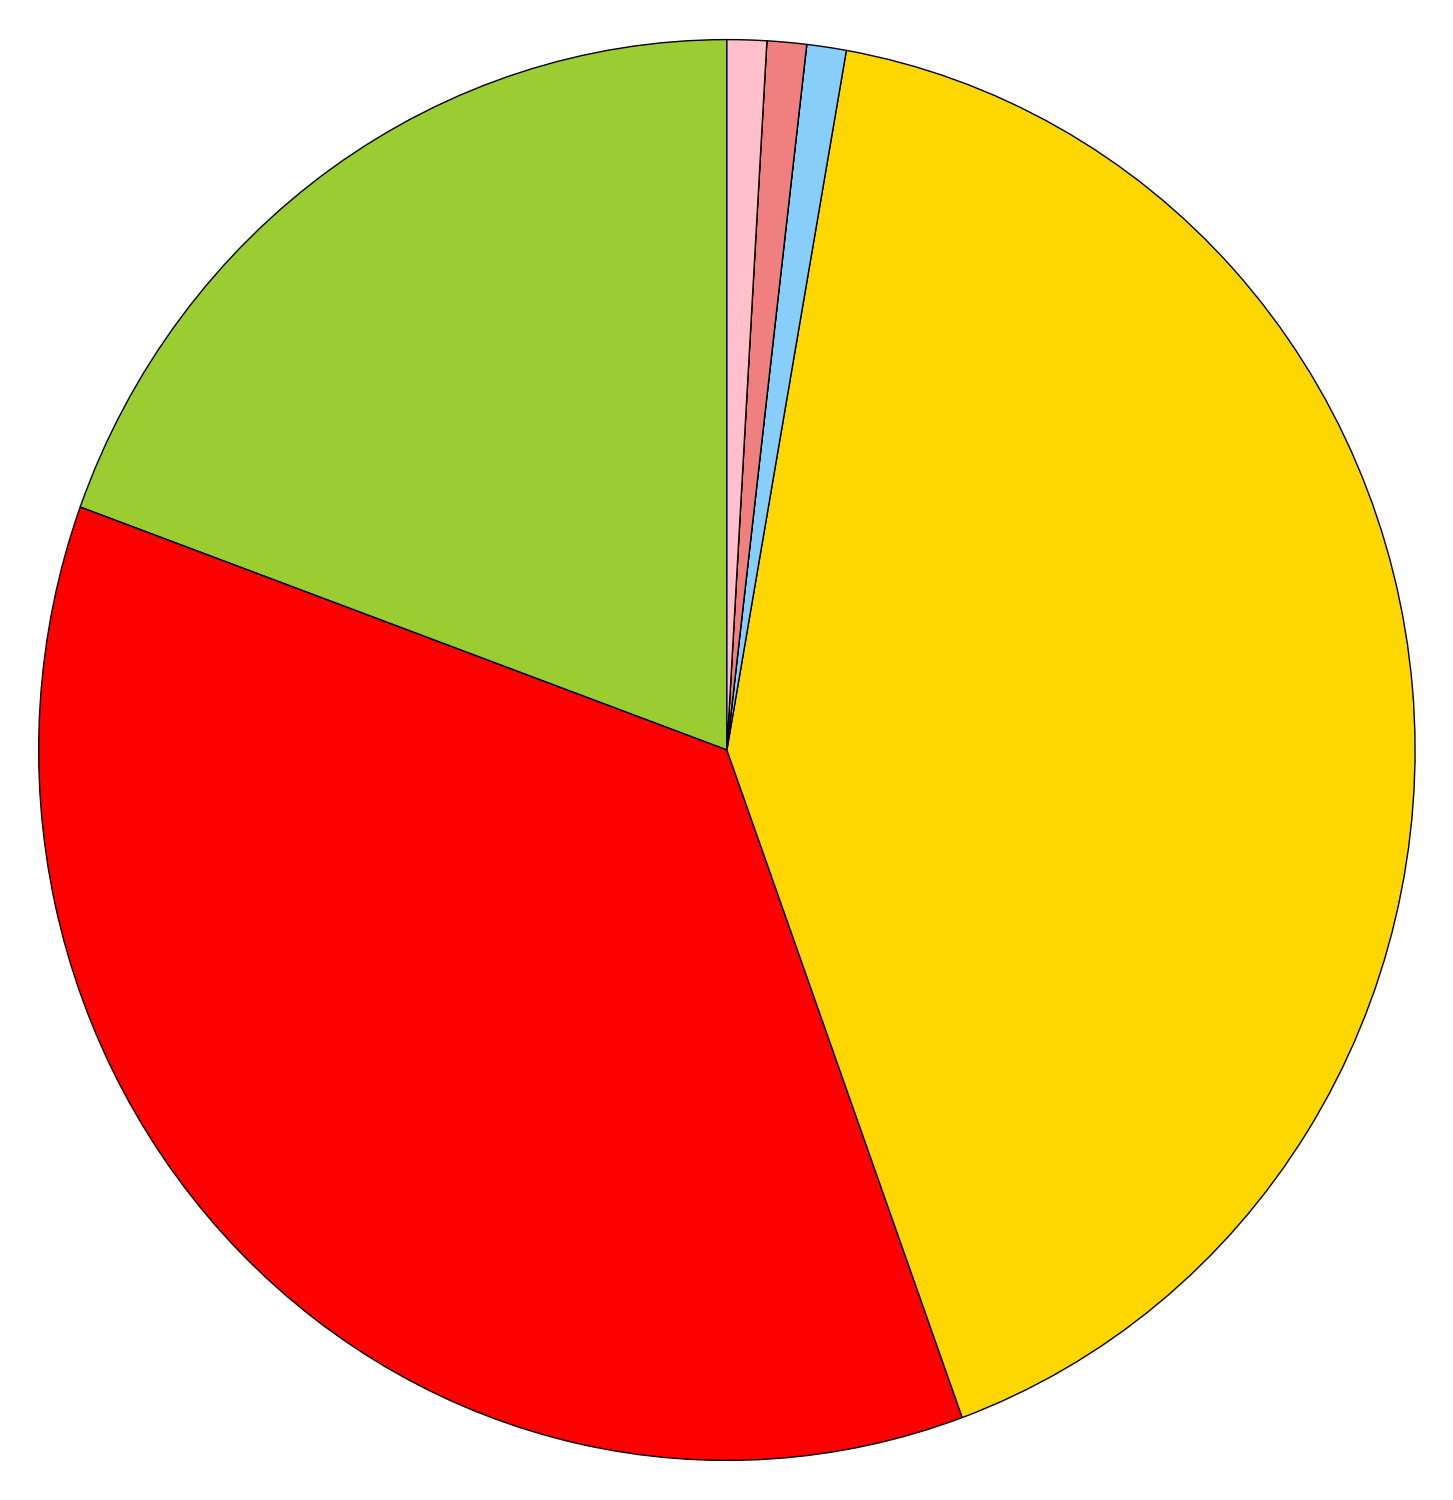
\includegraphics[width=\textwidth]{arousalALLMutInf}
    \caption{Mutual information}
  \end{subfigure}
  \hfill
  \begin{subfigure}[b]{0.3\textwidth}
    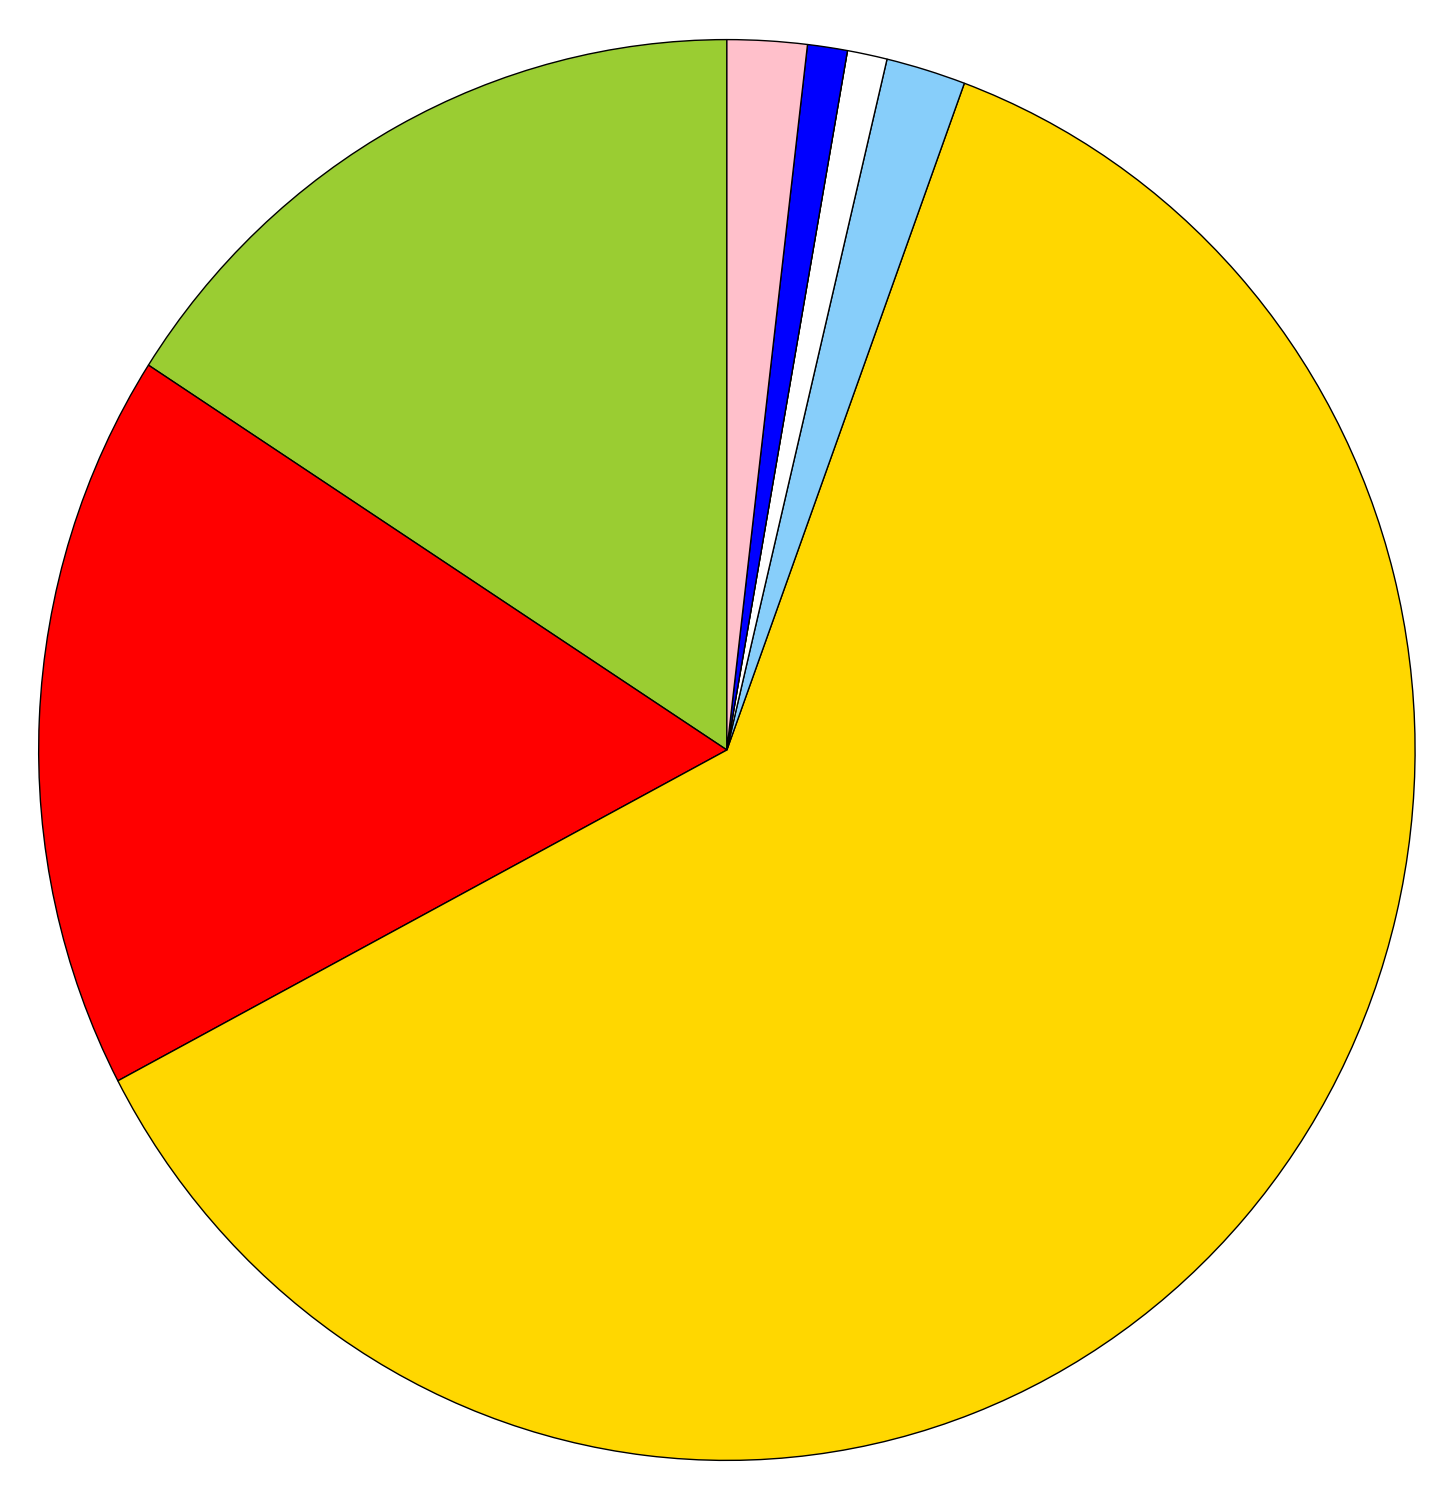
\includegraphics[width=\textwidth]{arousalALLdCorr}
    \caption{Distance Correlation}
  \end{subfigure}
  
  \begin{subfigure}[b]{0.3\textwidth}
    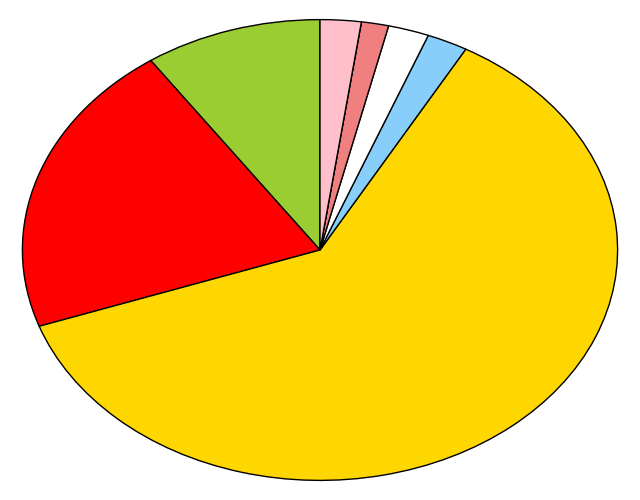
\includegraphics[width=\textwidth]{arousalALLANOVA}
    \caption{ANOVA}
  \end{subfigure}
  \hfill
  \begin{subfigure}[b]{0.3\textwidth}
    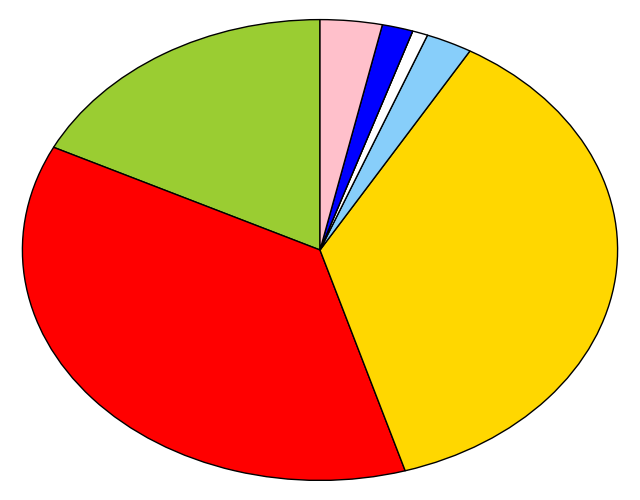
\includegraphics[width=\textwidth]{arousalALLLR}
    \caption{Linear regression}
  \end{subfigure}
  \hfill
  \begin{subfigure}[b]{0.3\textwidth}
    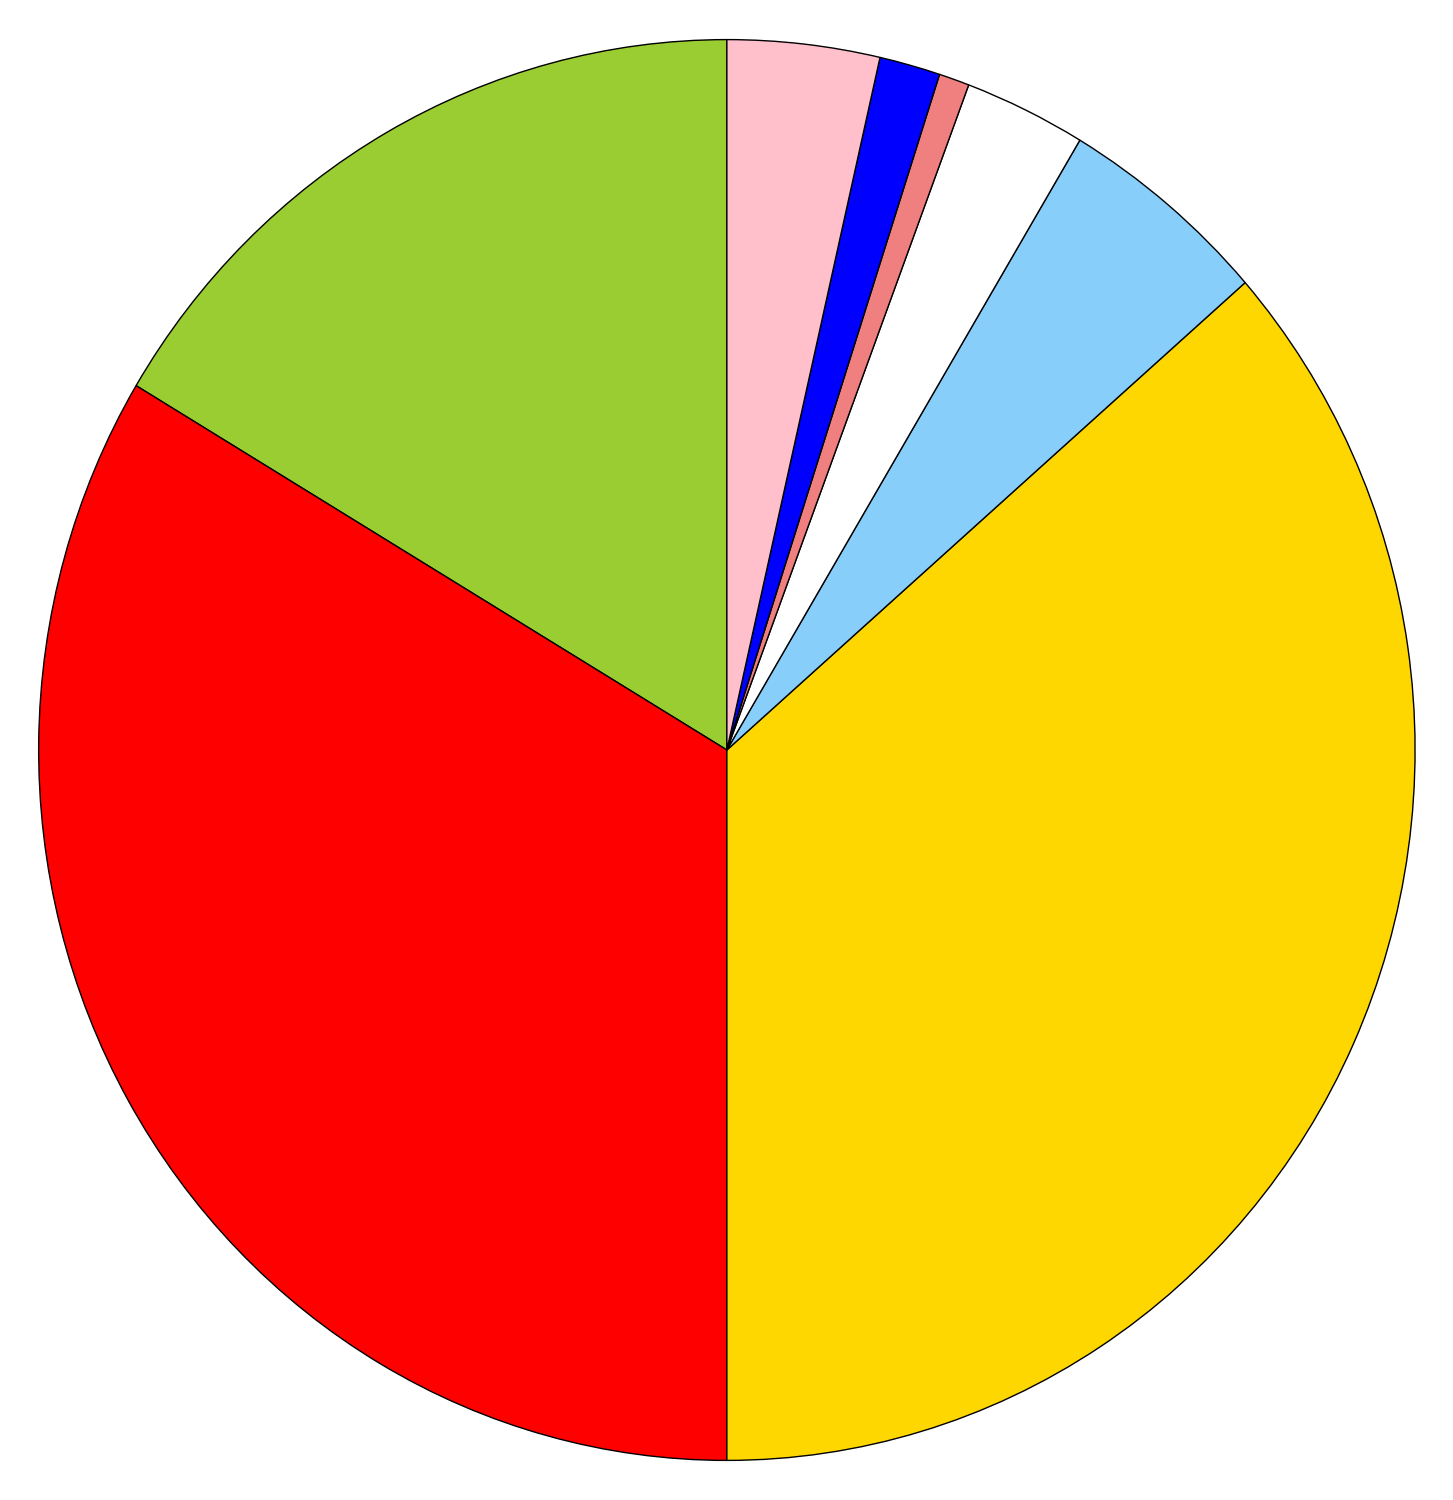
\includegraphics[width=\textwidth]{arousalALLSVM}
    \caption{SVM}
  \end{subfigure}
  
  \begin{subfigure}[b]{0.3\textwidth}
    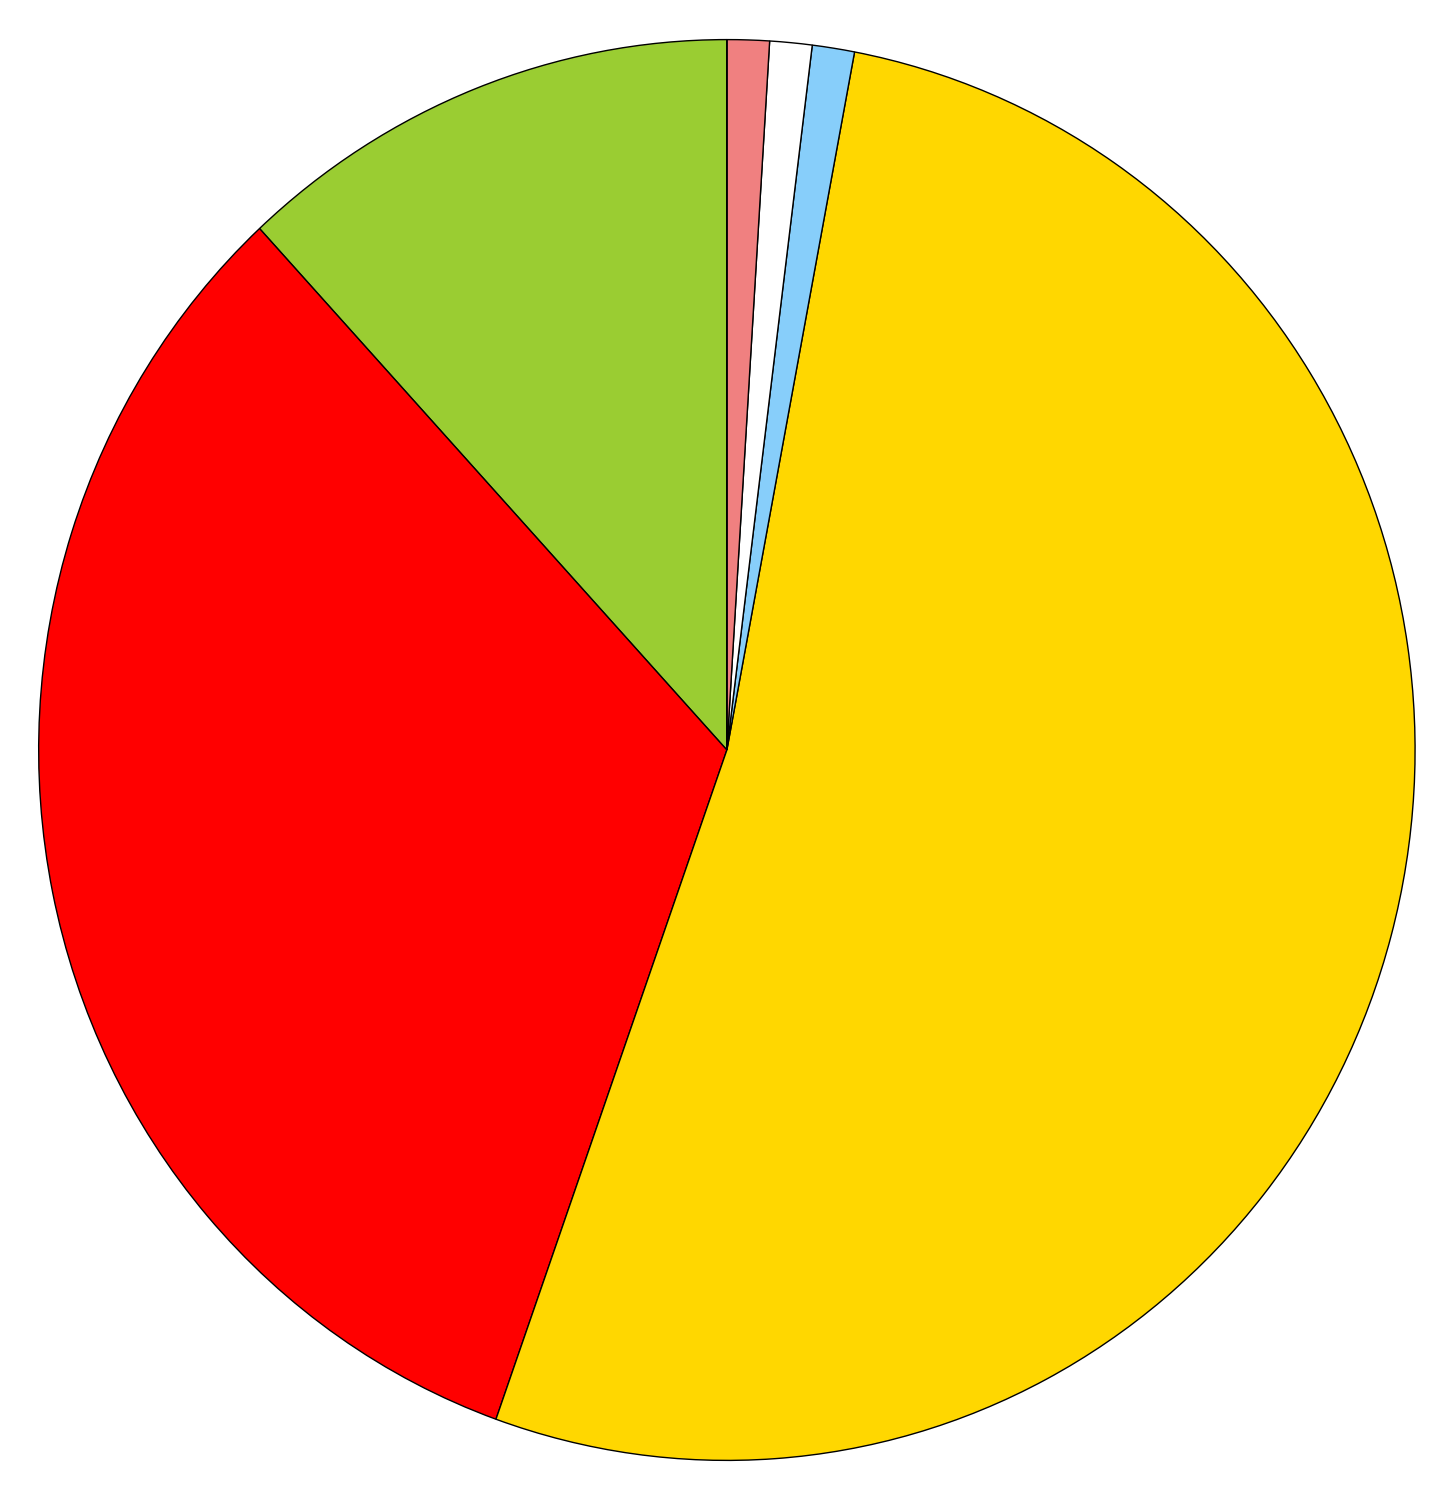
\includegraphics[width=\textwidth]{arousalALLLDA}
    \caption{LDA}
  \end{subfigure}
  \hfill
  \begin{subfigure}[b]{0.3\textwidth}
    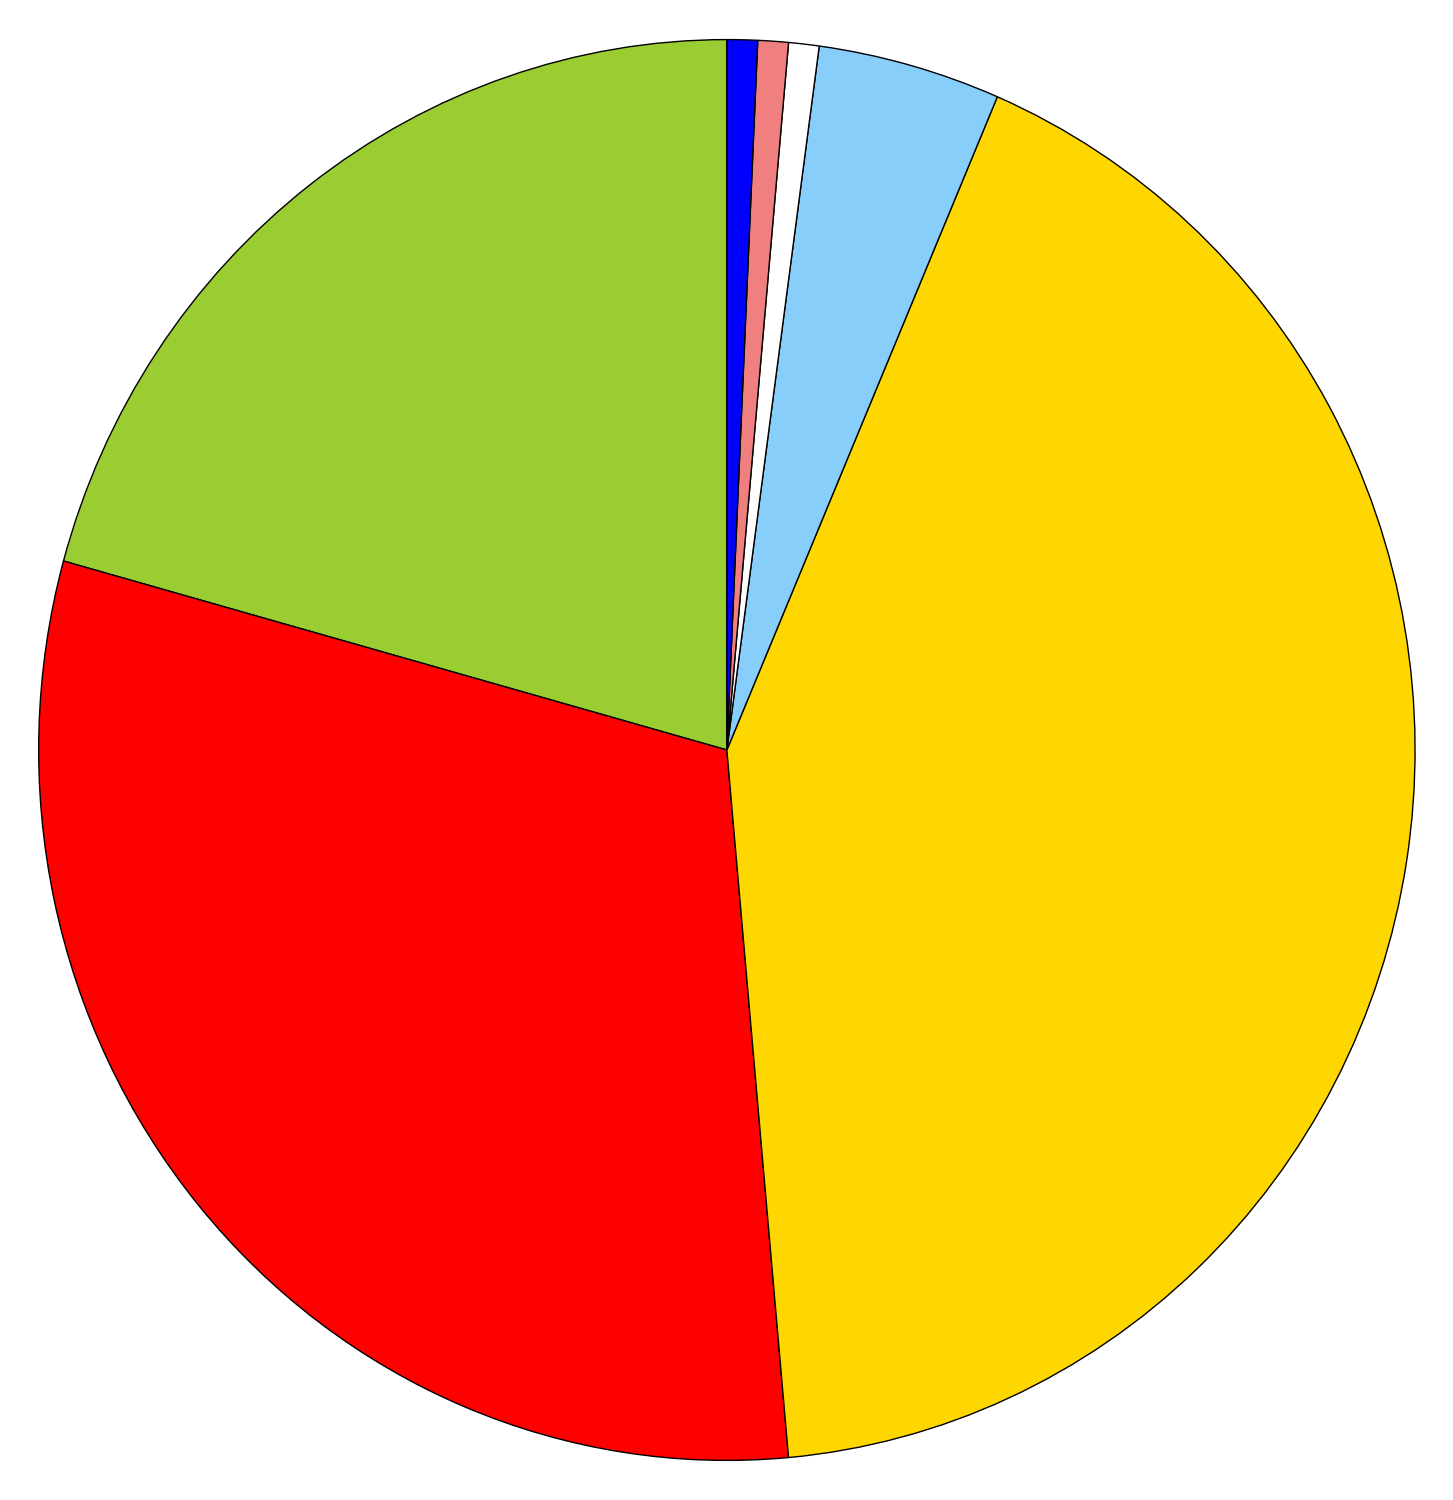
\includegraphics[width=\textwidth]{arousalALLL1}
    \caption{Lasso regression}
  \end{subfigure}
  \hfill
  \begin{subfigure}[b]{0.3\textwidth}
    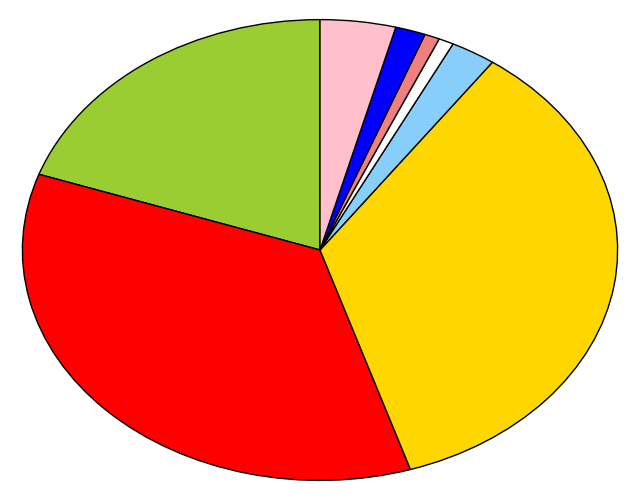
\includegraphics[width=\textwidth]{arousalALLL2}
    \caption{Ridge regression}
  \end{subfigure}
  
  \begin{subfigure}[b]{0.3\textwidth}
    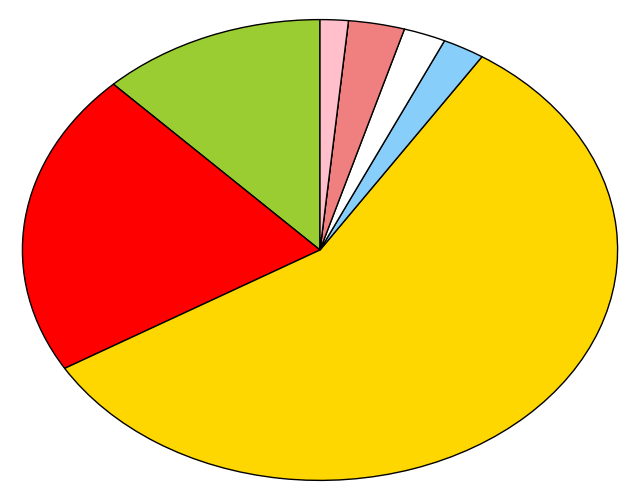
\includegraphics[width=\textwidth]{arousalALLRF}
    \caption{Random forests}
  \end{subfigure}
  \hfill
  \begin{subfigure}[b]{0.3\textwidth}
    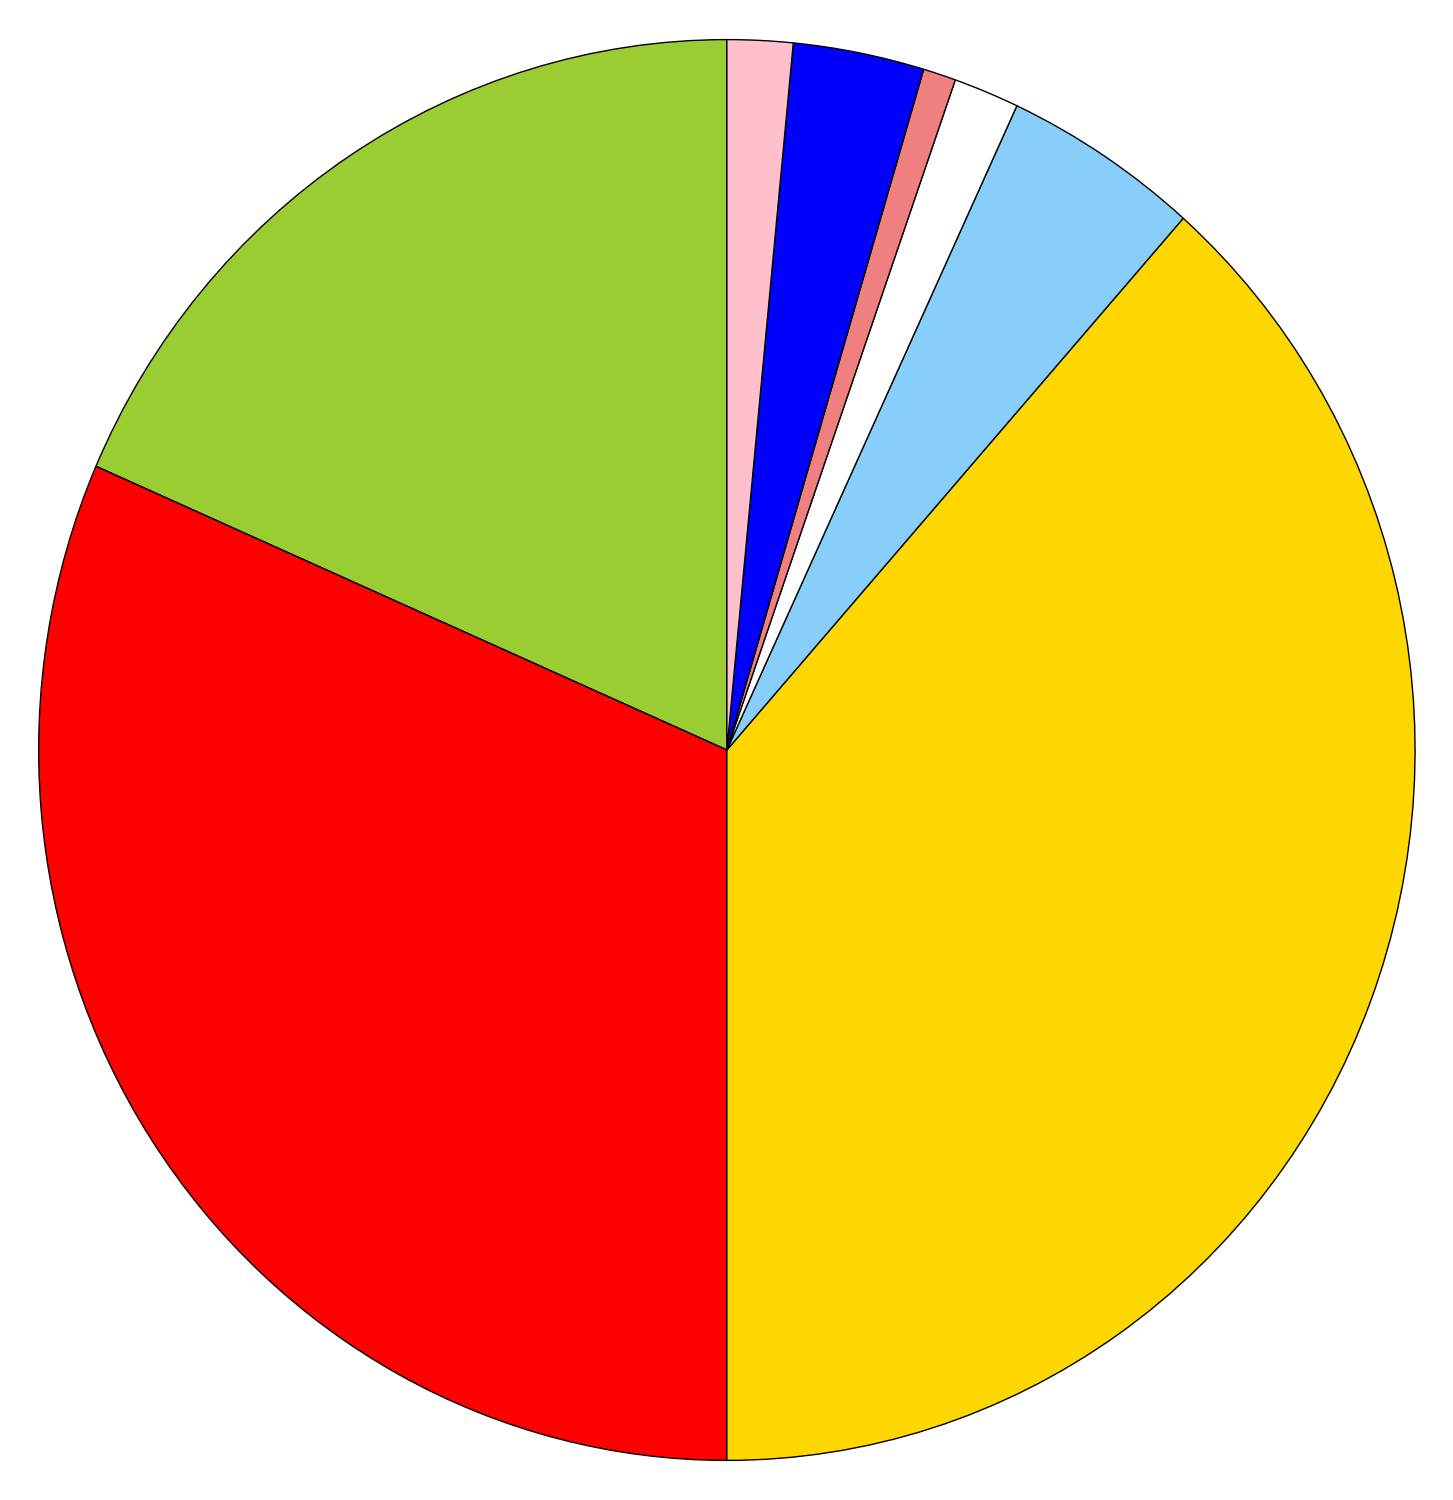
\includegraphics[width=\textwidth]{arousalALLPCA} %TODO 
    \caption{PCA}
  \end{subfigure}
  \hfill
  \begin{subfigure}[b]{0.3\textwidth}
    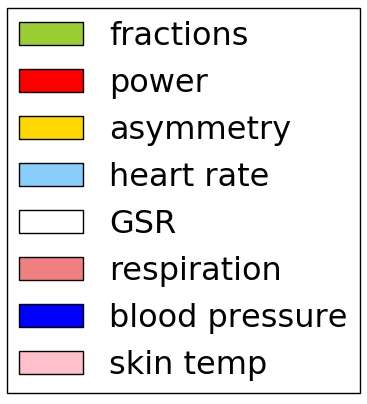
\includegraphics[width=\textwidth]{legend}
    \caption{Legend\label{arousalpieslegend}}
  \end{subfigure}
\end{figure}

\clearpage

\begin{figure}[!tbp]
  \centering
  \caption{Selection features for valence classification.\label{valencepies}}
  \begin{subfigure}[b]{0.3\textwidth}
    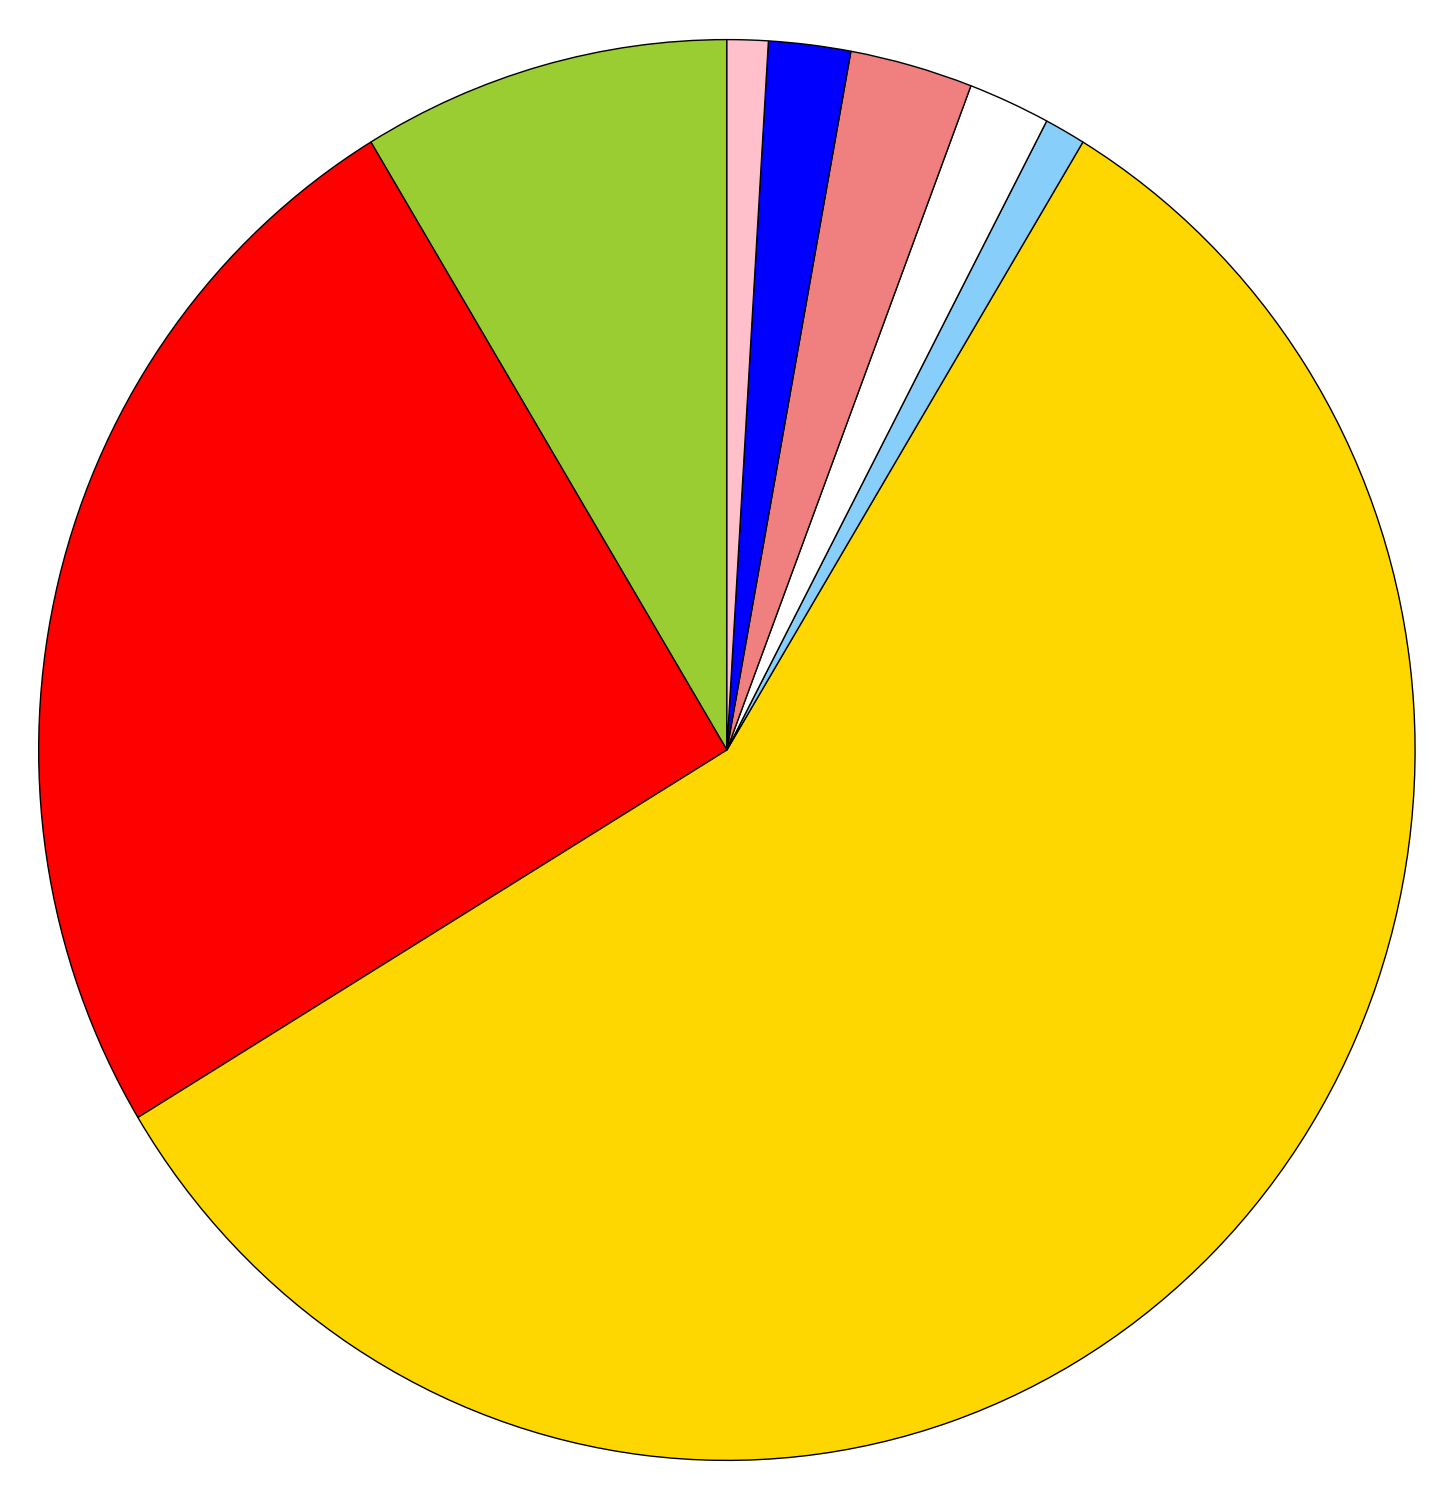
\includegraphics[width=\textwidth]{valenceALLpearsonR}
    \caption{Pearson correlation}
  \end{subfigure}
  \hfill
  \begin{subfigure}[b]{0.3\textwidth}
    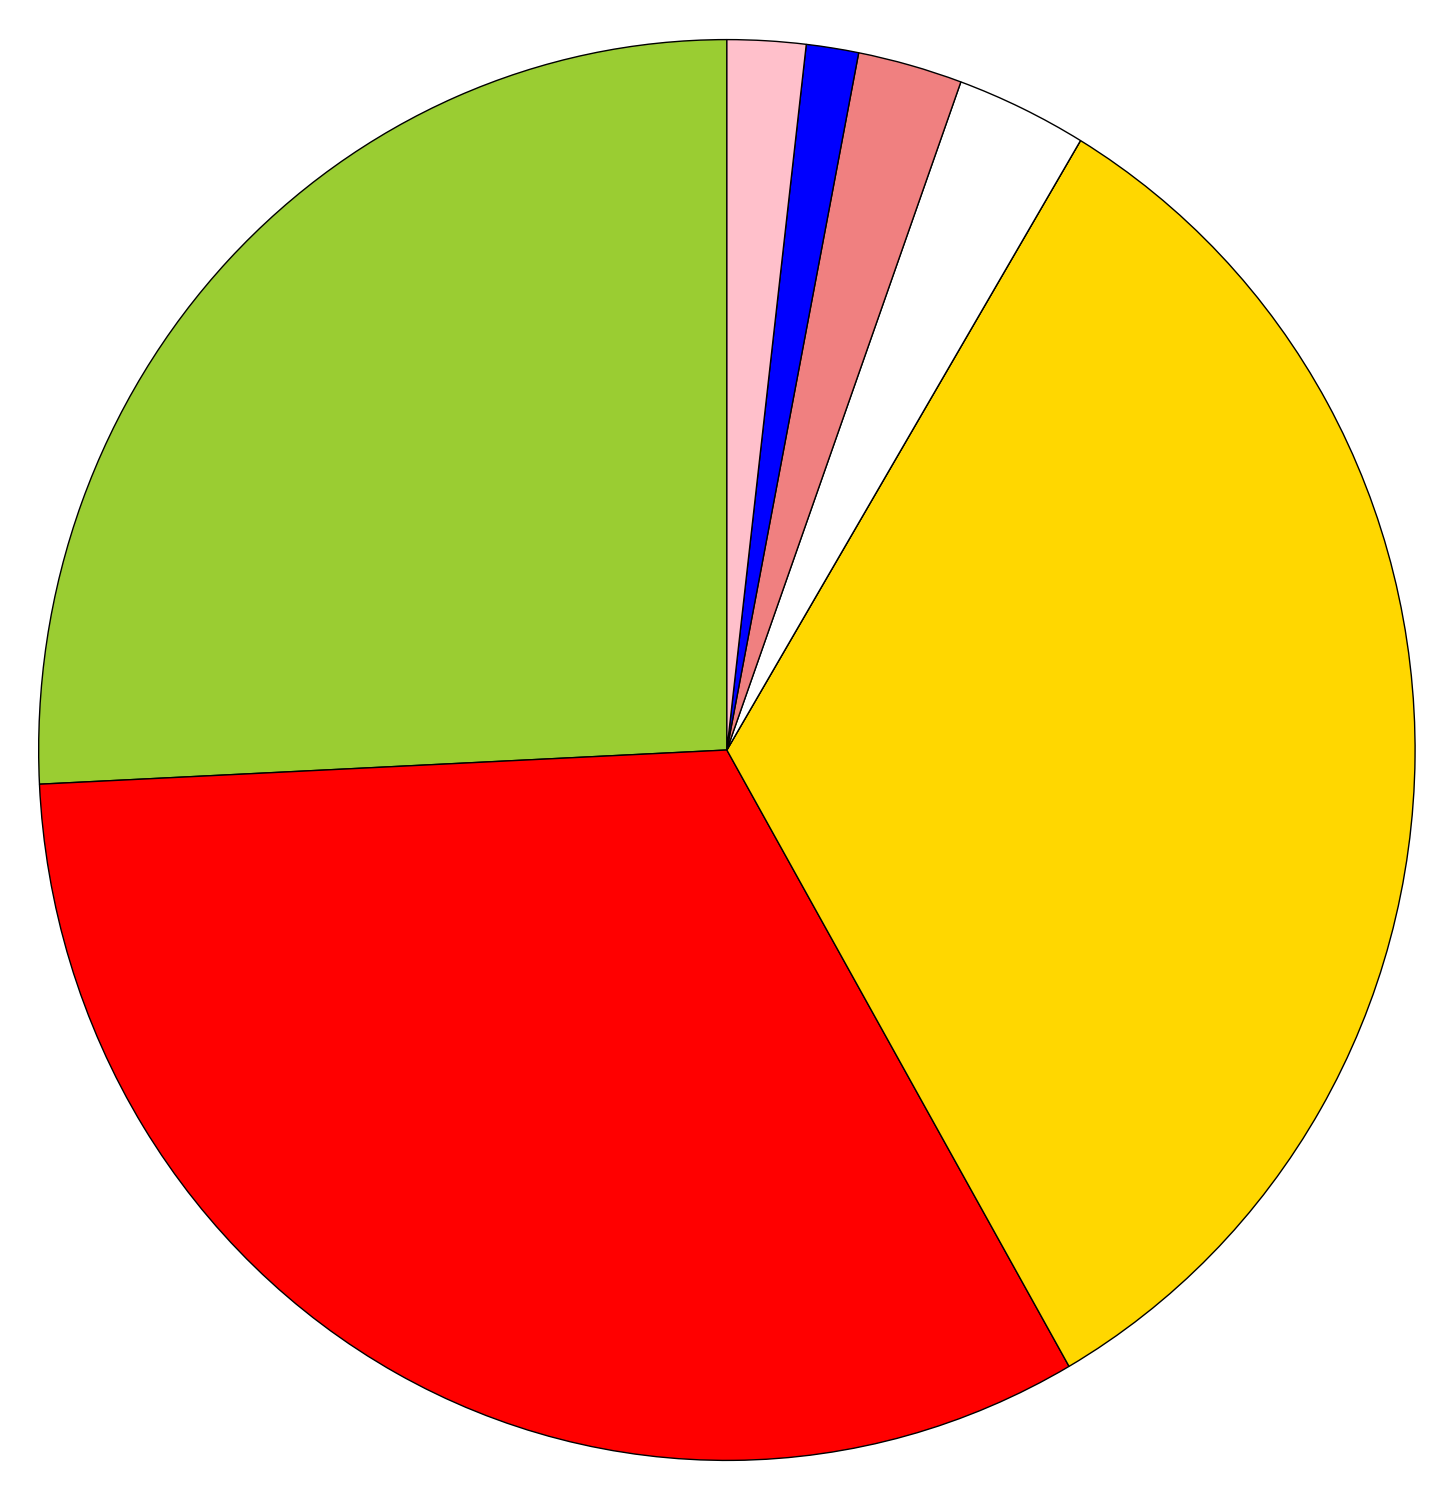
\includegraphics[width=\textwidth]{valenceALLMutInf}
    \caption{Mutual information}
  \end{subfigure}
  \hfill
  \begin{subfigure}[b]{0.3\textwidth}
    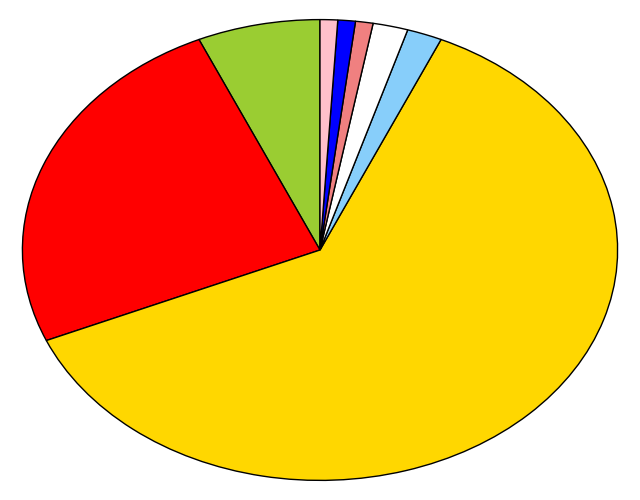
\includegraphics[width=\textwidth]{valenceALLdCorr}
    \caption{Distance Correlation}
  \end{subfigure}
  
  \begin{subfigure}[b]{0.3\textwidth}
    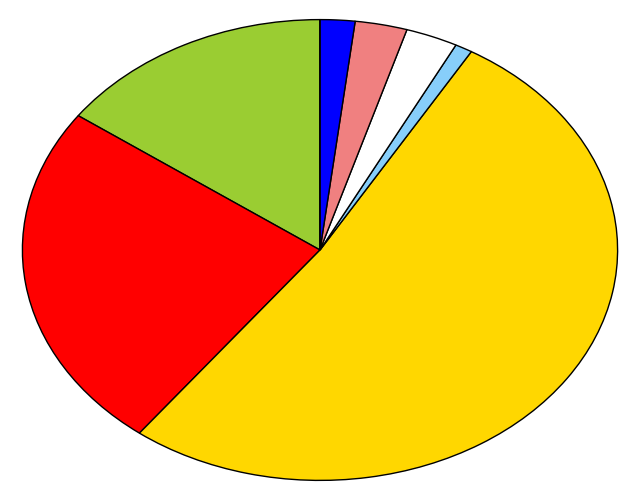
\includegraphics[width=\textwidth]{valenceALLANOVA}
    \caption{ANOVA}
  \end{subfigure}
  \hfill
  \begin{subfigure}[b]{0.3\textwidth}
    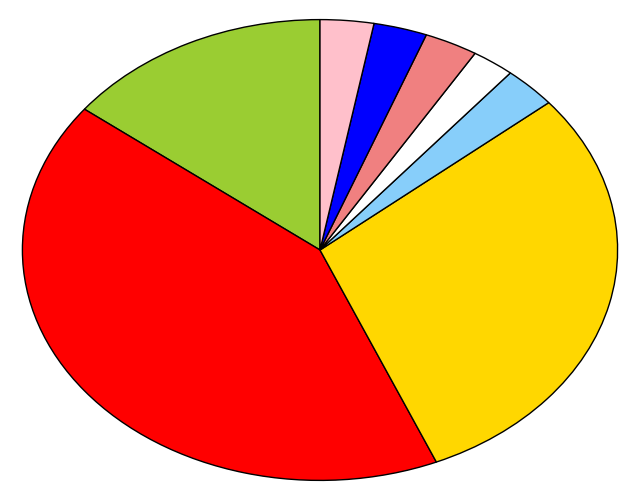
\includegraphics[width=\textwidth]{valenceALLLR}
    \caption{Linear regression}
  \end{subfigure}
  \hfill
  \begin{subfigure}[b]{0.3\textwidth}
    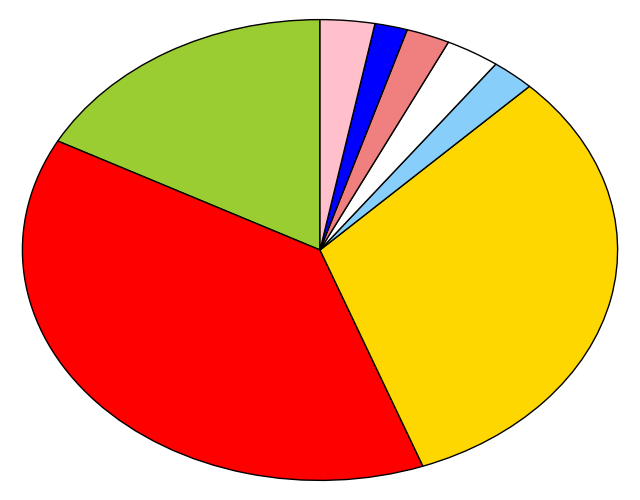
\includegraphics[width=\textwidth]{valenceALLSVM}
    \caption{SVM}
  \end{subfigure}
  
  \begin{subfigure}[b]{0.3\textwidth}
    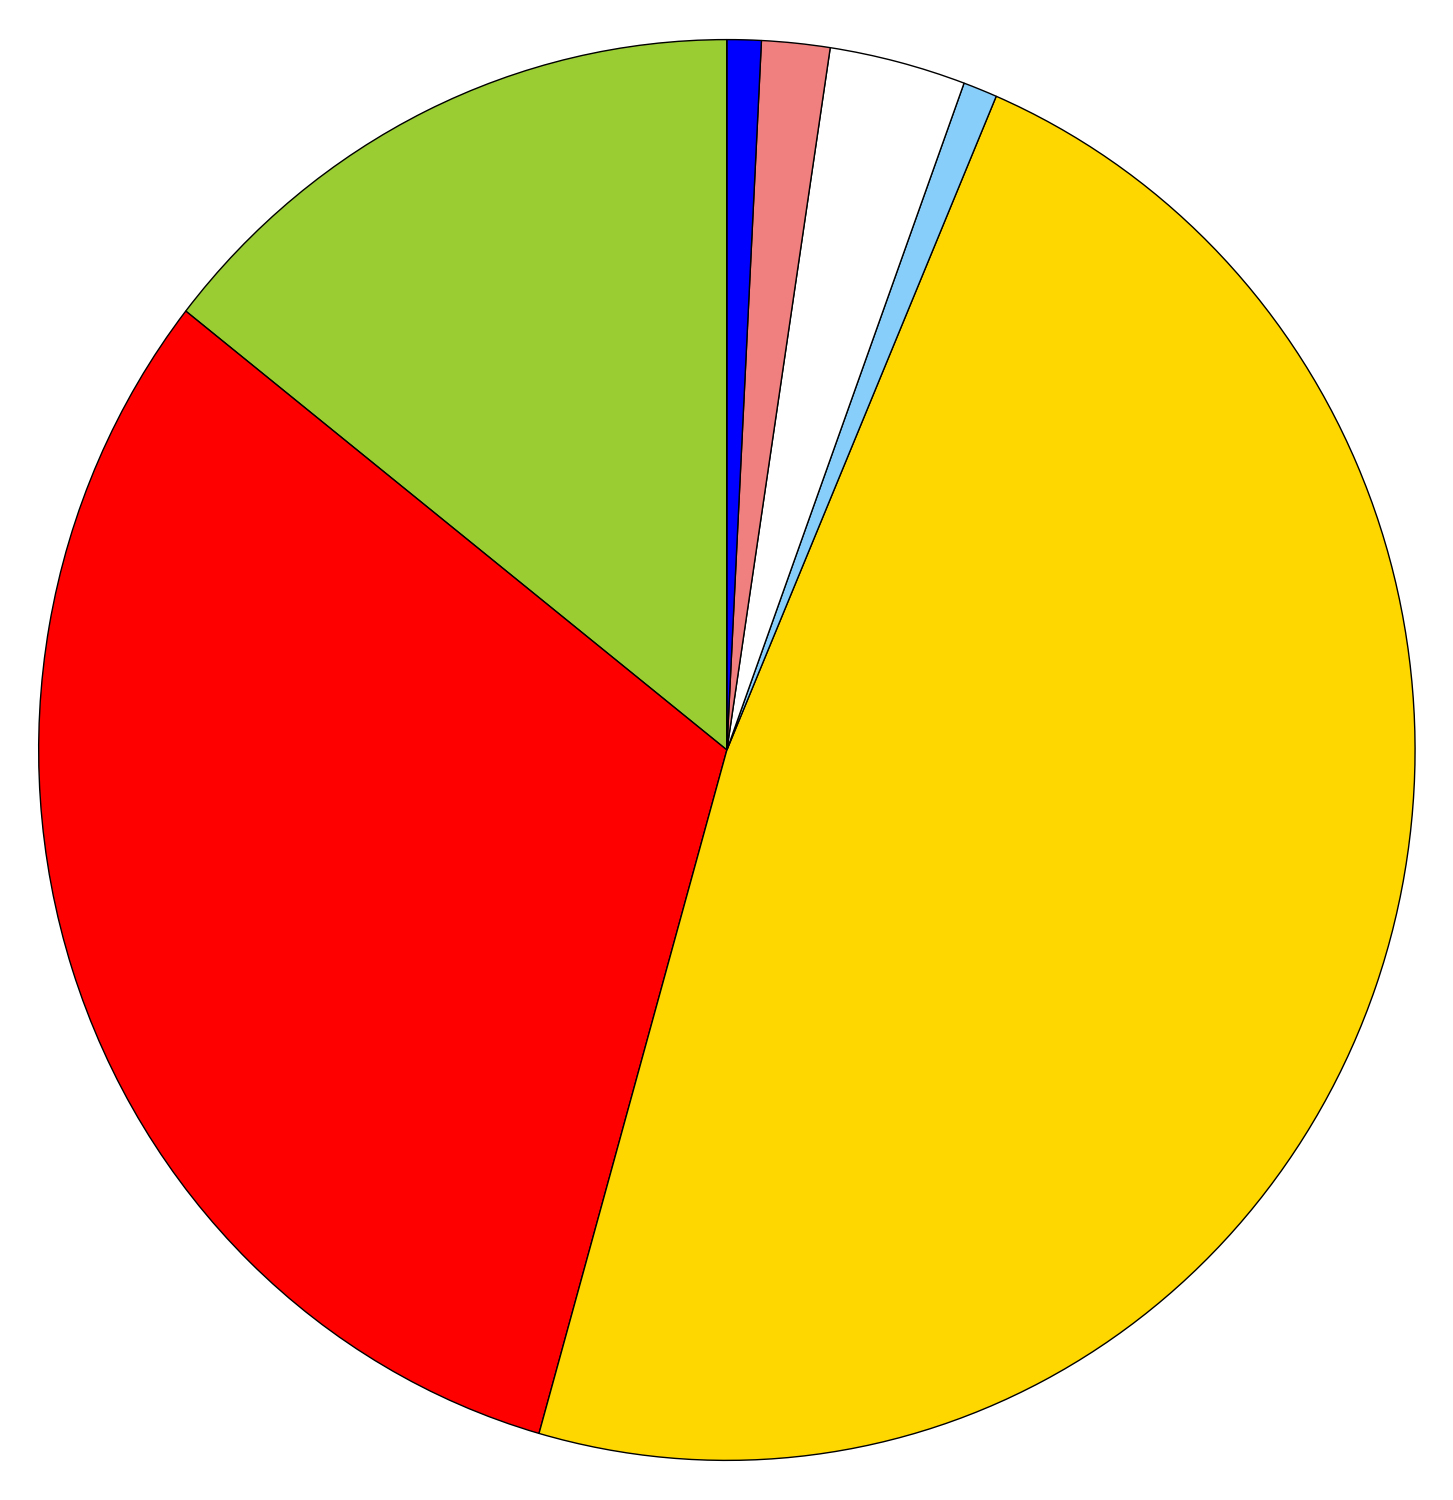
\includegraphics[width=\textwidth]{valenceALLLDA}
    \caption{LDA}
  \end{subfigure}
  \hfill
  \begin{subfigure}[b]{0.3\textwidth}
    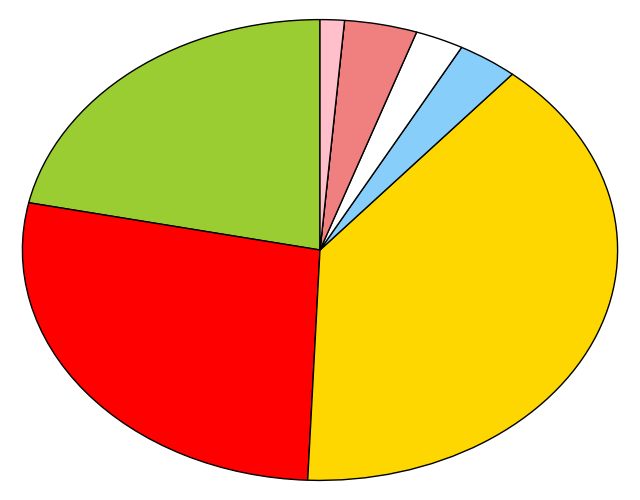
\includegraphics[width=\textwidth]{valenceALLL1}
    \caption{Lasso regression}
  \end{subfigure}
  \hfill
  \begin{subfigure}[b]{0.3\textwidth}
    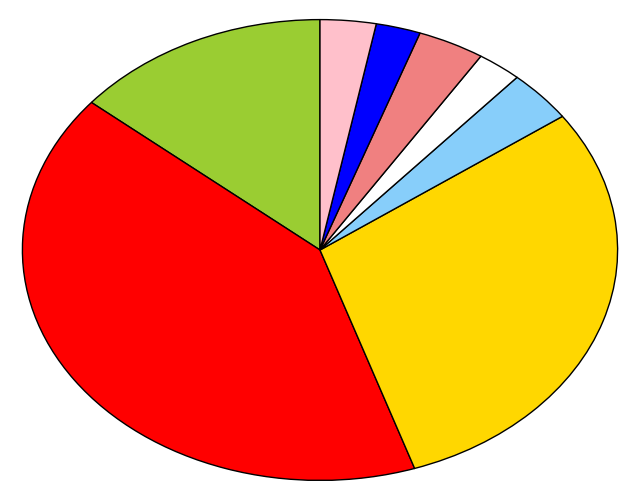
\includegraphics[width=\textwidth]{valenceALLL2}
    \caption{Ridge regression}
  \end{subfigure}
  
  \begin{subfigure}[b]{0.3\textwidth}
    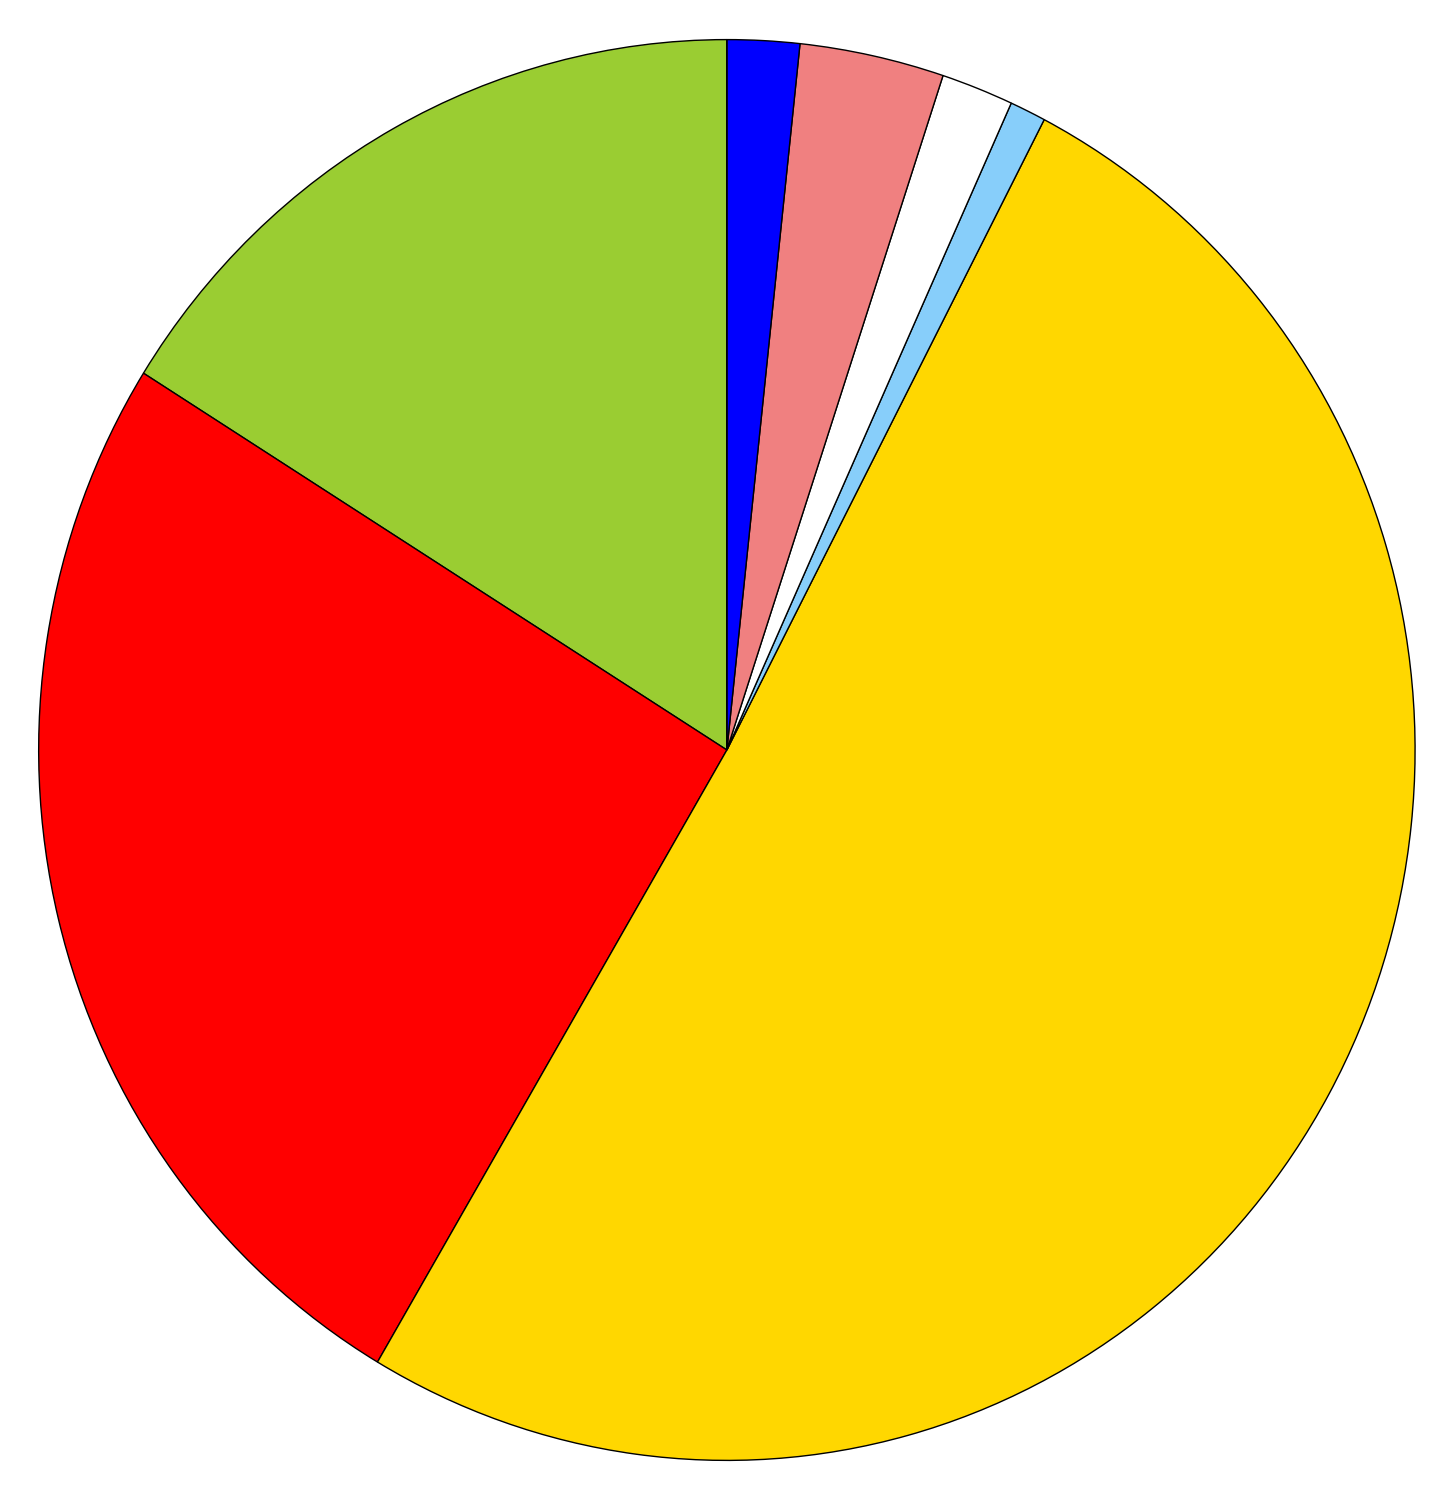
\includegraphics[width=\textwidth]{valenceALLRF}
    \caption{Random forests}
  \end{subfigure}
  \hfill
  \begin{subfigure}[b]{0.3\textwidth}
    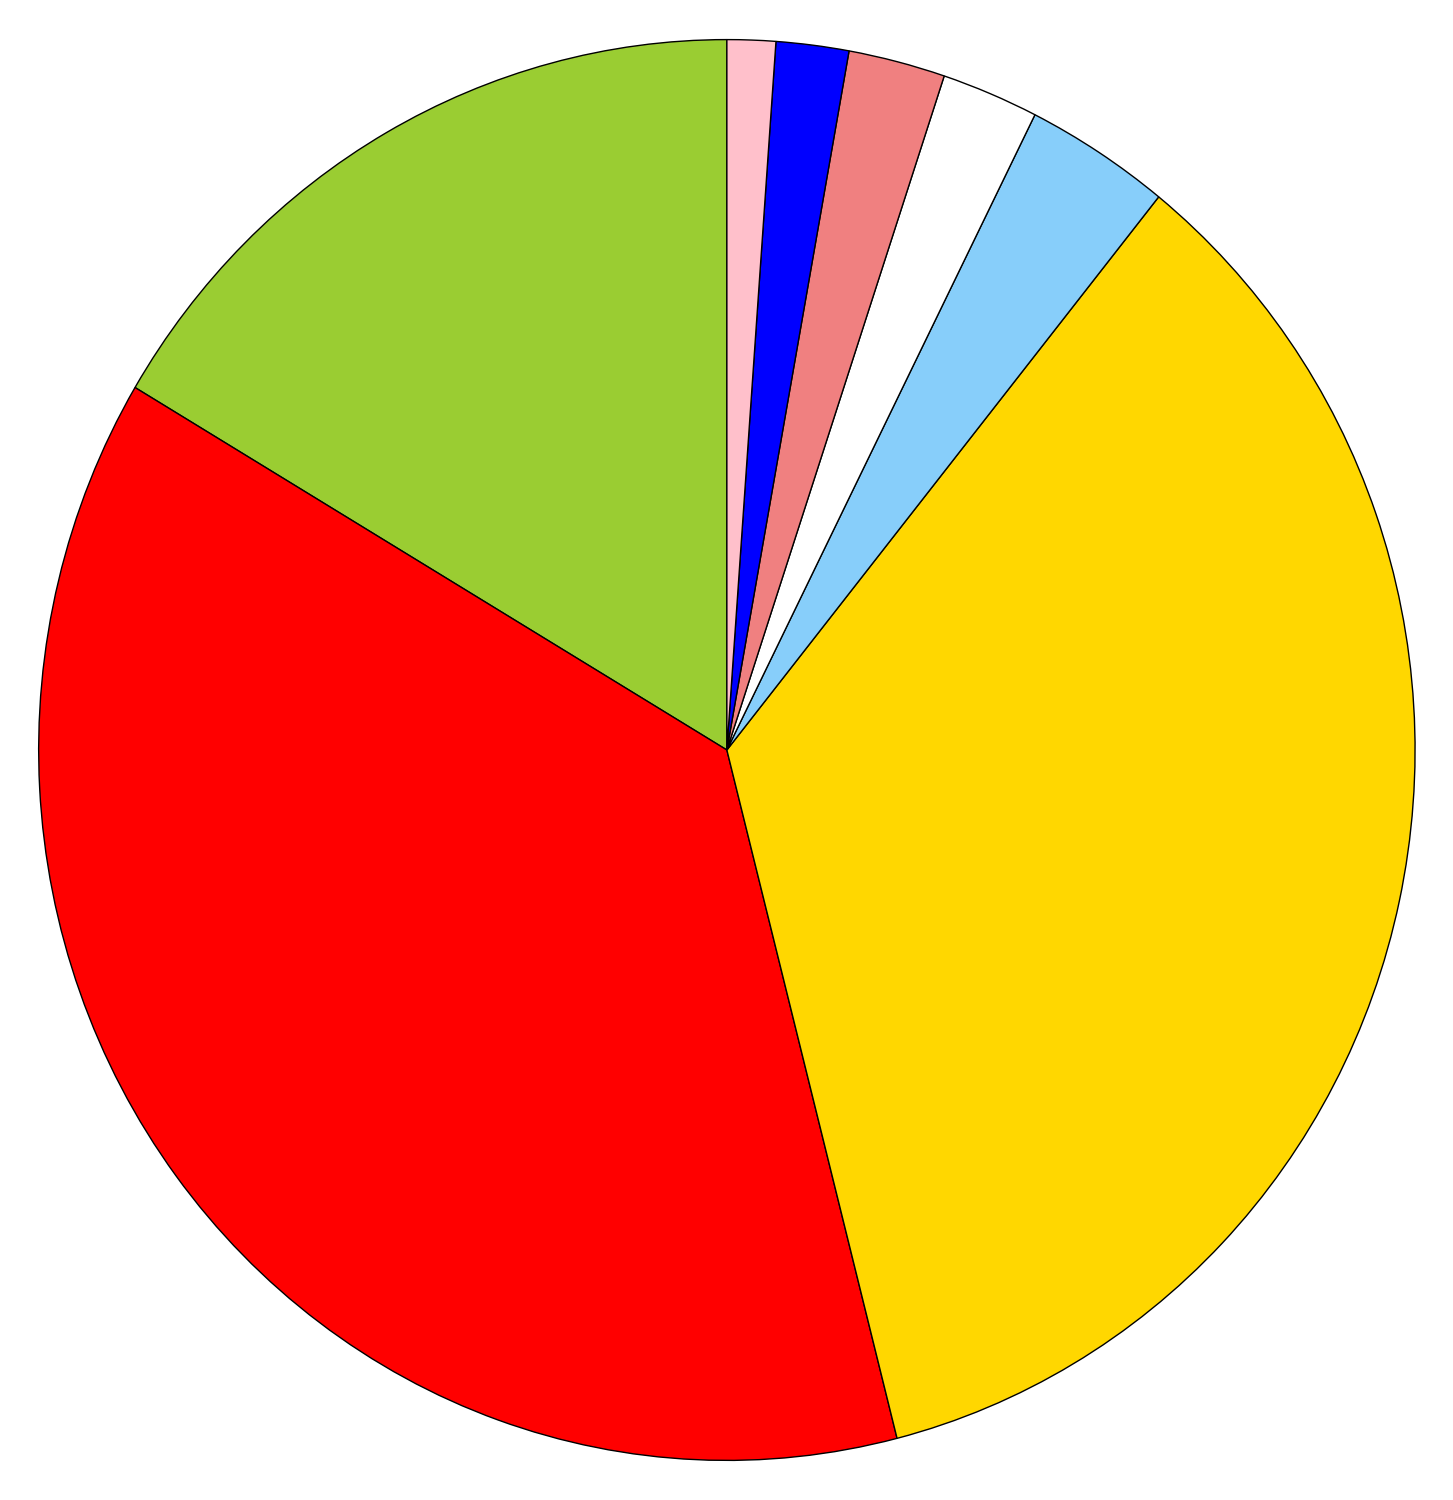
\includegraphics[width=\textwidth]{valenceALLPCA} %TODO 
    \caption{PCA}
  \end{subfigure}
  \hfill
  \begin{subfigure}[b]{0.3\textwidth}
    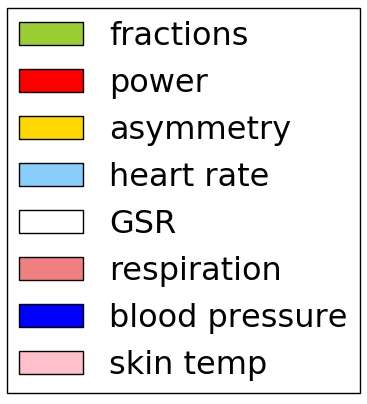
\includegraphics[width=\textwidth]{legend}
    \caption{Legend\label{valencepieslegend}}
  \end{subfigure}
\end{figure}
\clearpage

The fact that the non-EEG features are rarely chose indicates that they are less important. In an attempt to further investigate the difference between EEG features and non-EEG features, the performance of three different feature sets was compared. The first feature set is the previously used features set with all possible features. The second and third feature sets contained only EEG and non-EEG features respectively. The feature selection was done with random forest, as this method had the best average performance, as well as the best correlations. 

\npar

The resulting performances of these different features sets is displayed in Figure \ref{arousalphyeegall} for arousal and in Figure \ref{valencephyeegall} for valence.

\mijnfiguur{width=1.\textwidth}{arousalphyeegall}{The performance of arousal prediction for all, EEG and non-EEG features.}

\mijnfiguur{width=1.\textwidth}{valencephyeegall}{The performance of valence prediction for all, EEG and non-EEG features.}

It is clear that for both valence and arousal, the average test performances are lower in case only non-EEG features are used. However the difference was not significant. %TODO p-value

\npar 

Next for each of the three feature sets, a comparison of the selected features was made. This will give more insight into which EEG and which non-EEG features are important. As you can see on Figure \ref{arousalEEGpies} for arousal and Figure \ref{valenceEEGpies}, displayed on the following pages, the features are again mostly asymmetry features, followed by the power features. The fraction only give limited insight. The EEG and ALL set have similar performances, because they both use very similar features.

\npar

In case that only non-EEG features are used, the selected features are from different categories. This is shown in Figure \ref{arousalnon-EEGpies} for arousal and Figure \ref{valencenon-EEGpies} for valence. Heart rate seems to be the most valuable feature for arousal. Additionally, the first selected feature for arousal is often the GSR, which measure how much perspiration a person has.
For valence though, there is no clear winner overall. However heart rate and GSR are often picked as the first feature.

\clearpage
\begin{figure}[!tbp]
  \centering
  \caption{Selection features for arousal classification, using only EEG features.\label{arousalEEGpies}}
  \begin{subfigure}[b]{0.3\textwidth}
    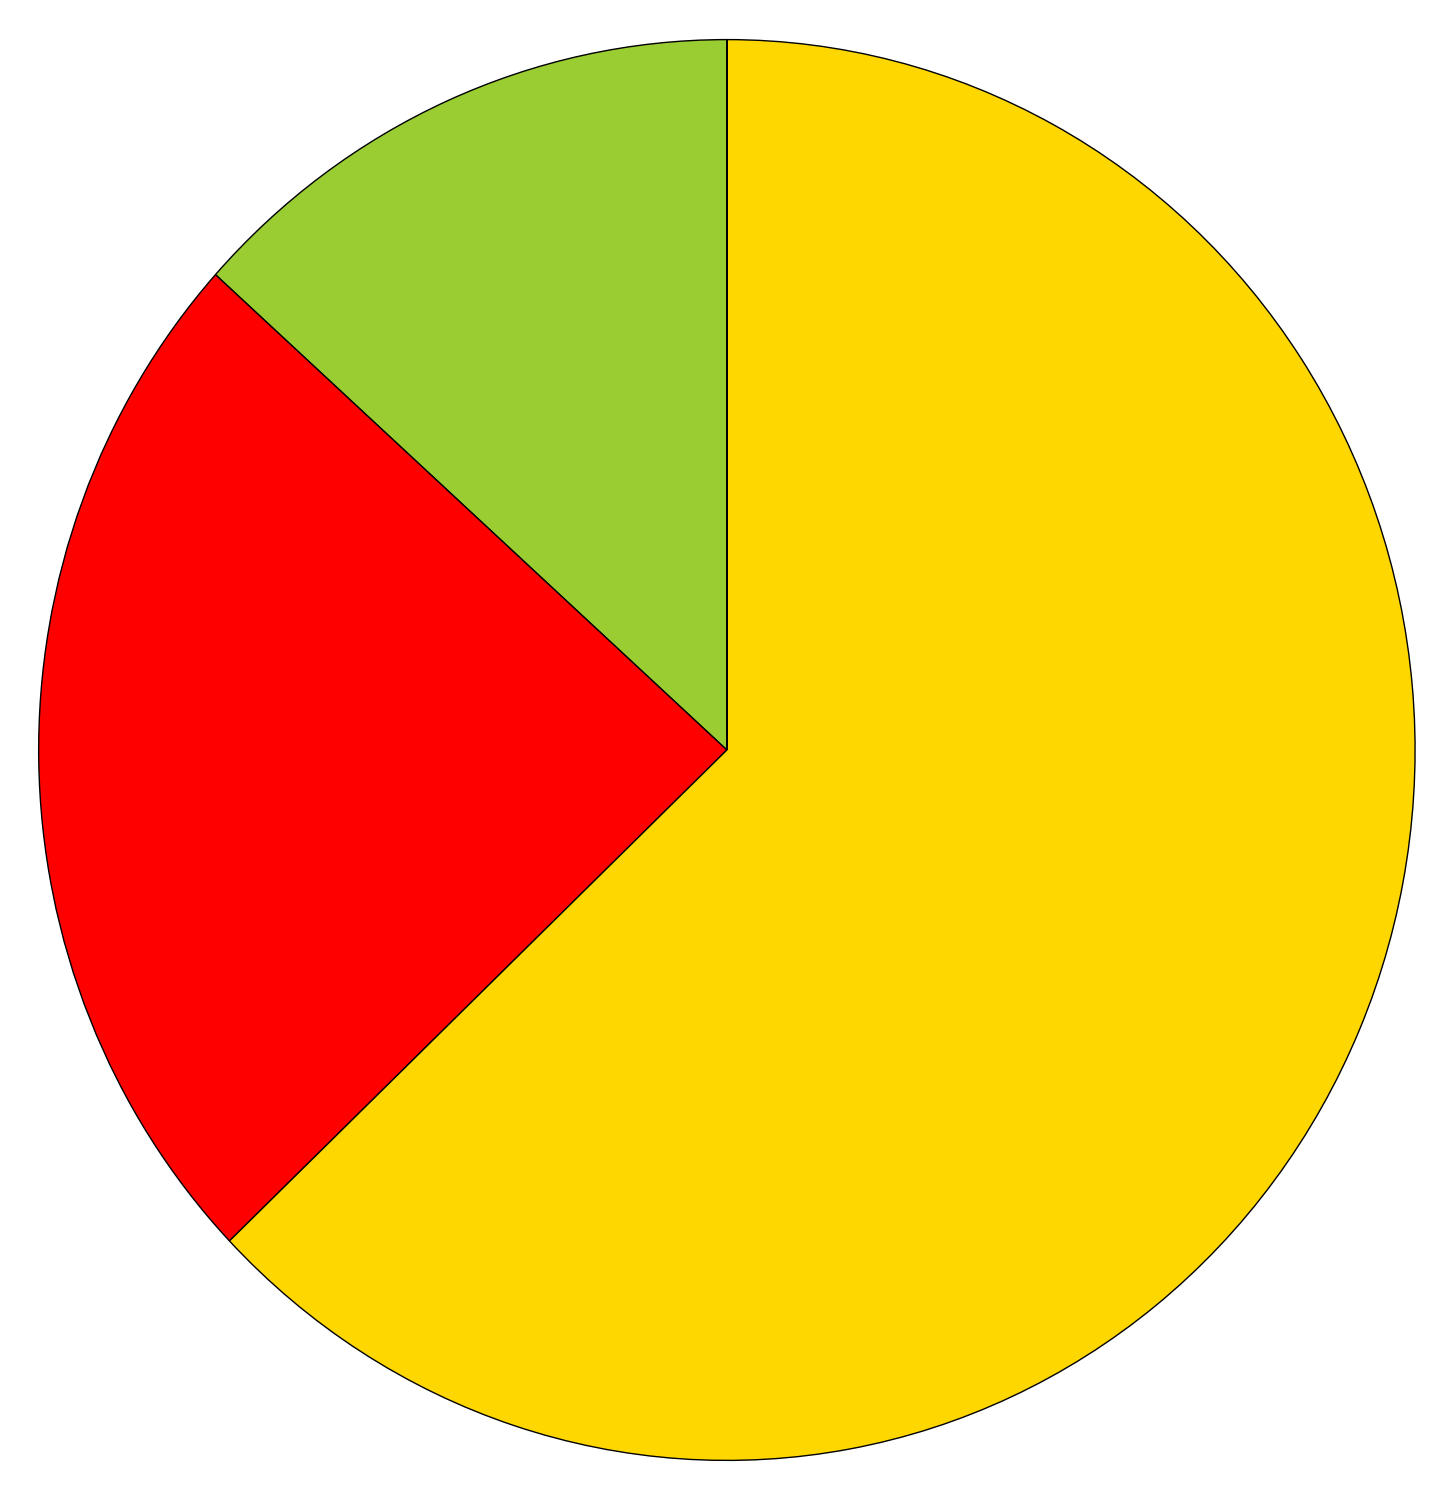
\includegraphics[width=\textwidth]{arousalEEGpearsonR}
    \caption{Pearson correlation}
  \end{subfigure}
  \hfill
  \begin{subfigure}[b]{0.3\textwidth}
    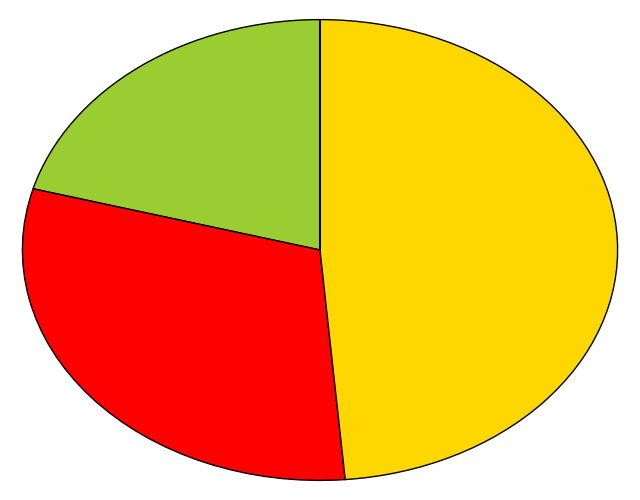
\includegraphics[width=\textwidth]{arousalEEGMutInf}
    \caption{Mutual information}
  \end{subfigure}
  \hfill
  \begin{subfigure}[b]{0.3\textwidth}
    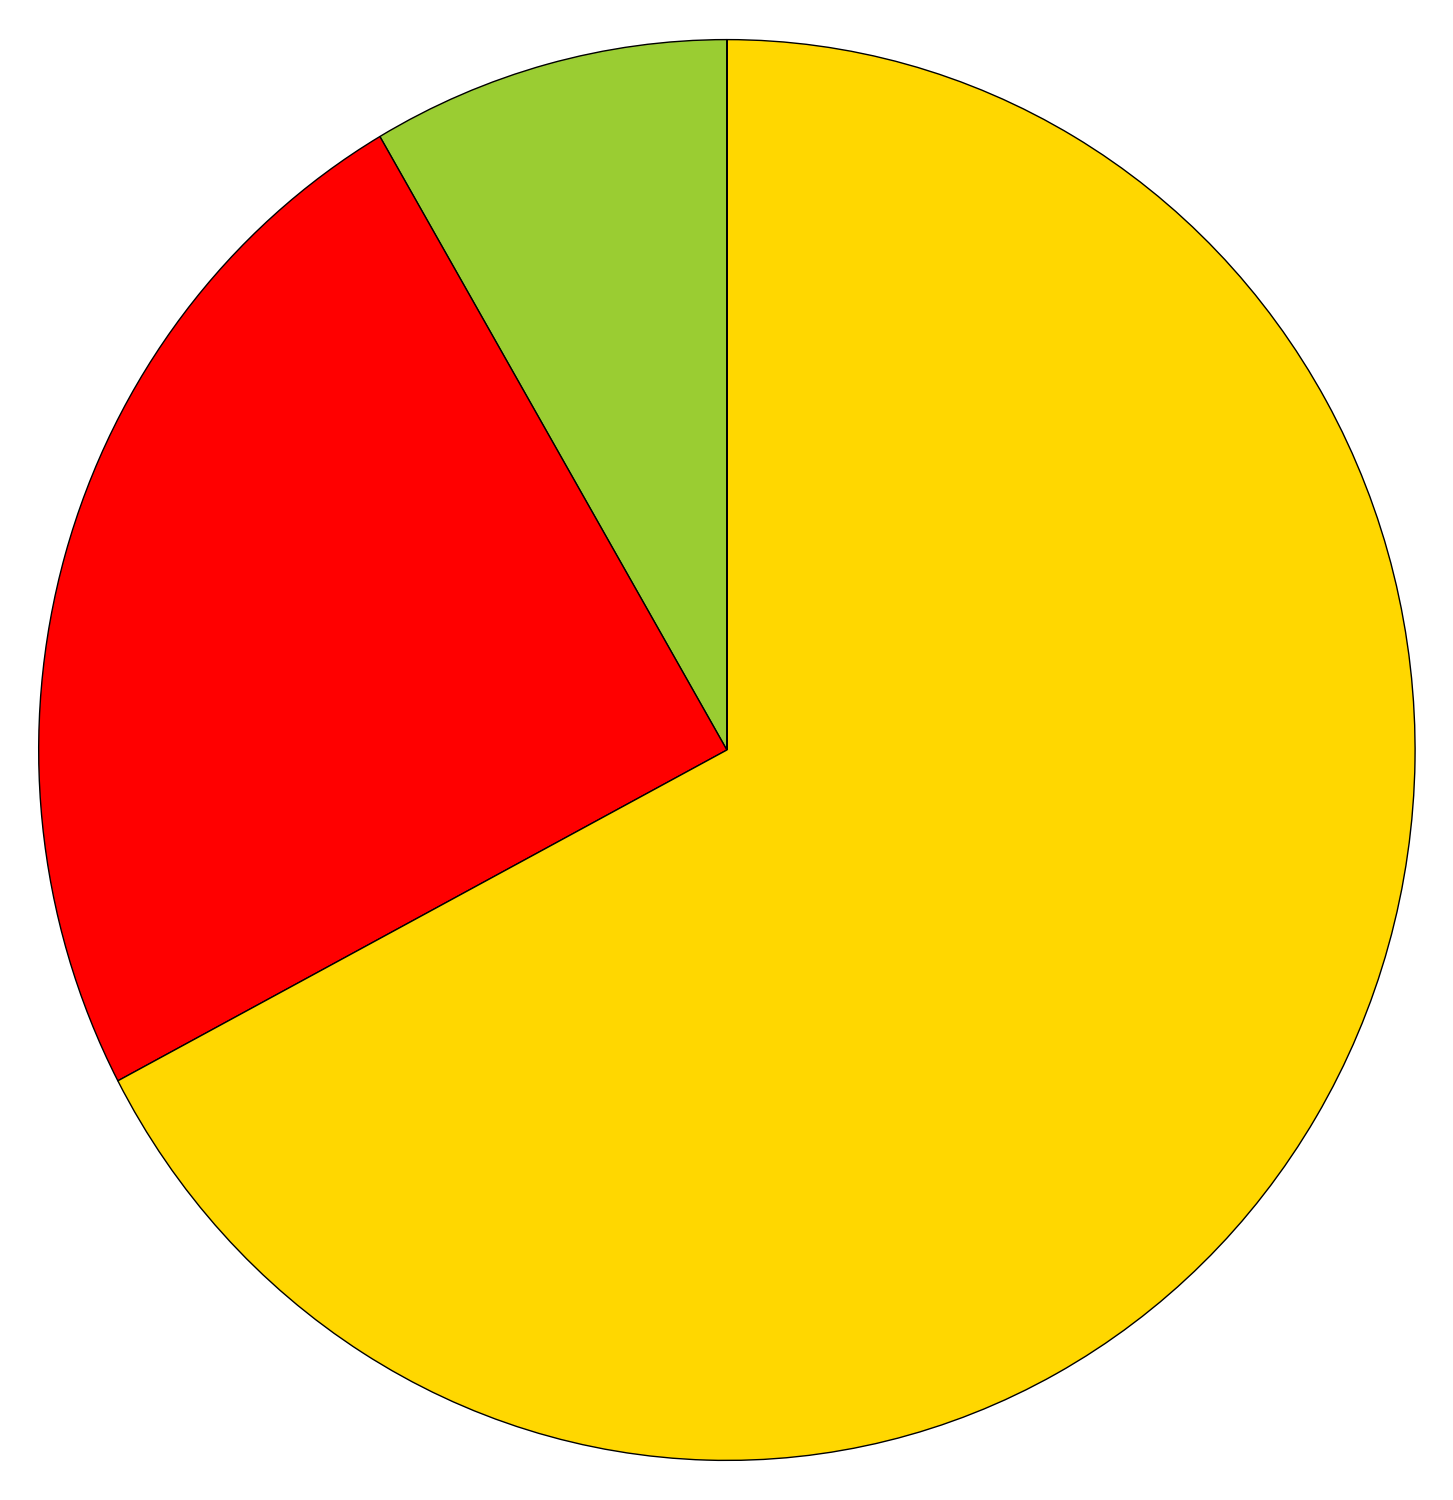
\includegraphics[width=\textwidth]{arousalEEGdCorr}
    \caption{Distance Correlation}
  \end{subfigure}
  
  \begin{subfigure}[b]{0.3\textwidth}
    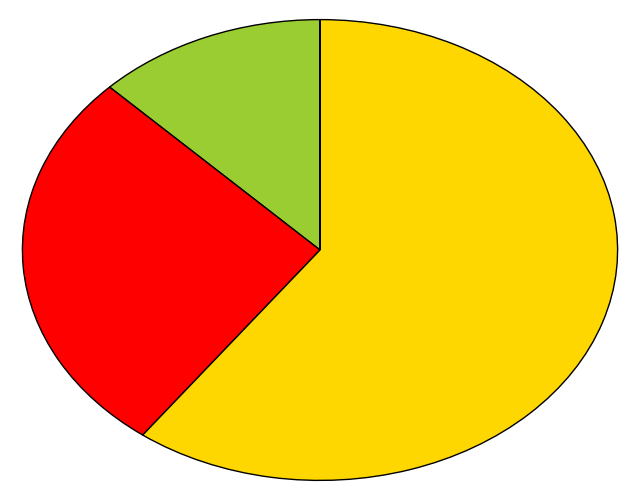
\includegraphics[width=\textwidth]{arousalEEGANOVA}
    \caption{ANOVA}
  \end{subfigure}
  \hfill
  \begin{subfigure}[b]{0.3\textwidth}
    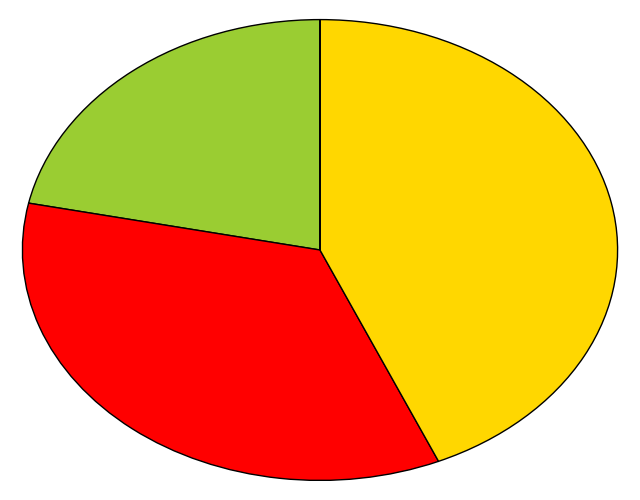
\includegraphics[width=\textwidth]{arousalEEGLR}
    \caption{Linear regression}
  \end{subfigure}
  \hfill
  \begin{subfigure}[b]{0.3\textwidth}
    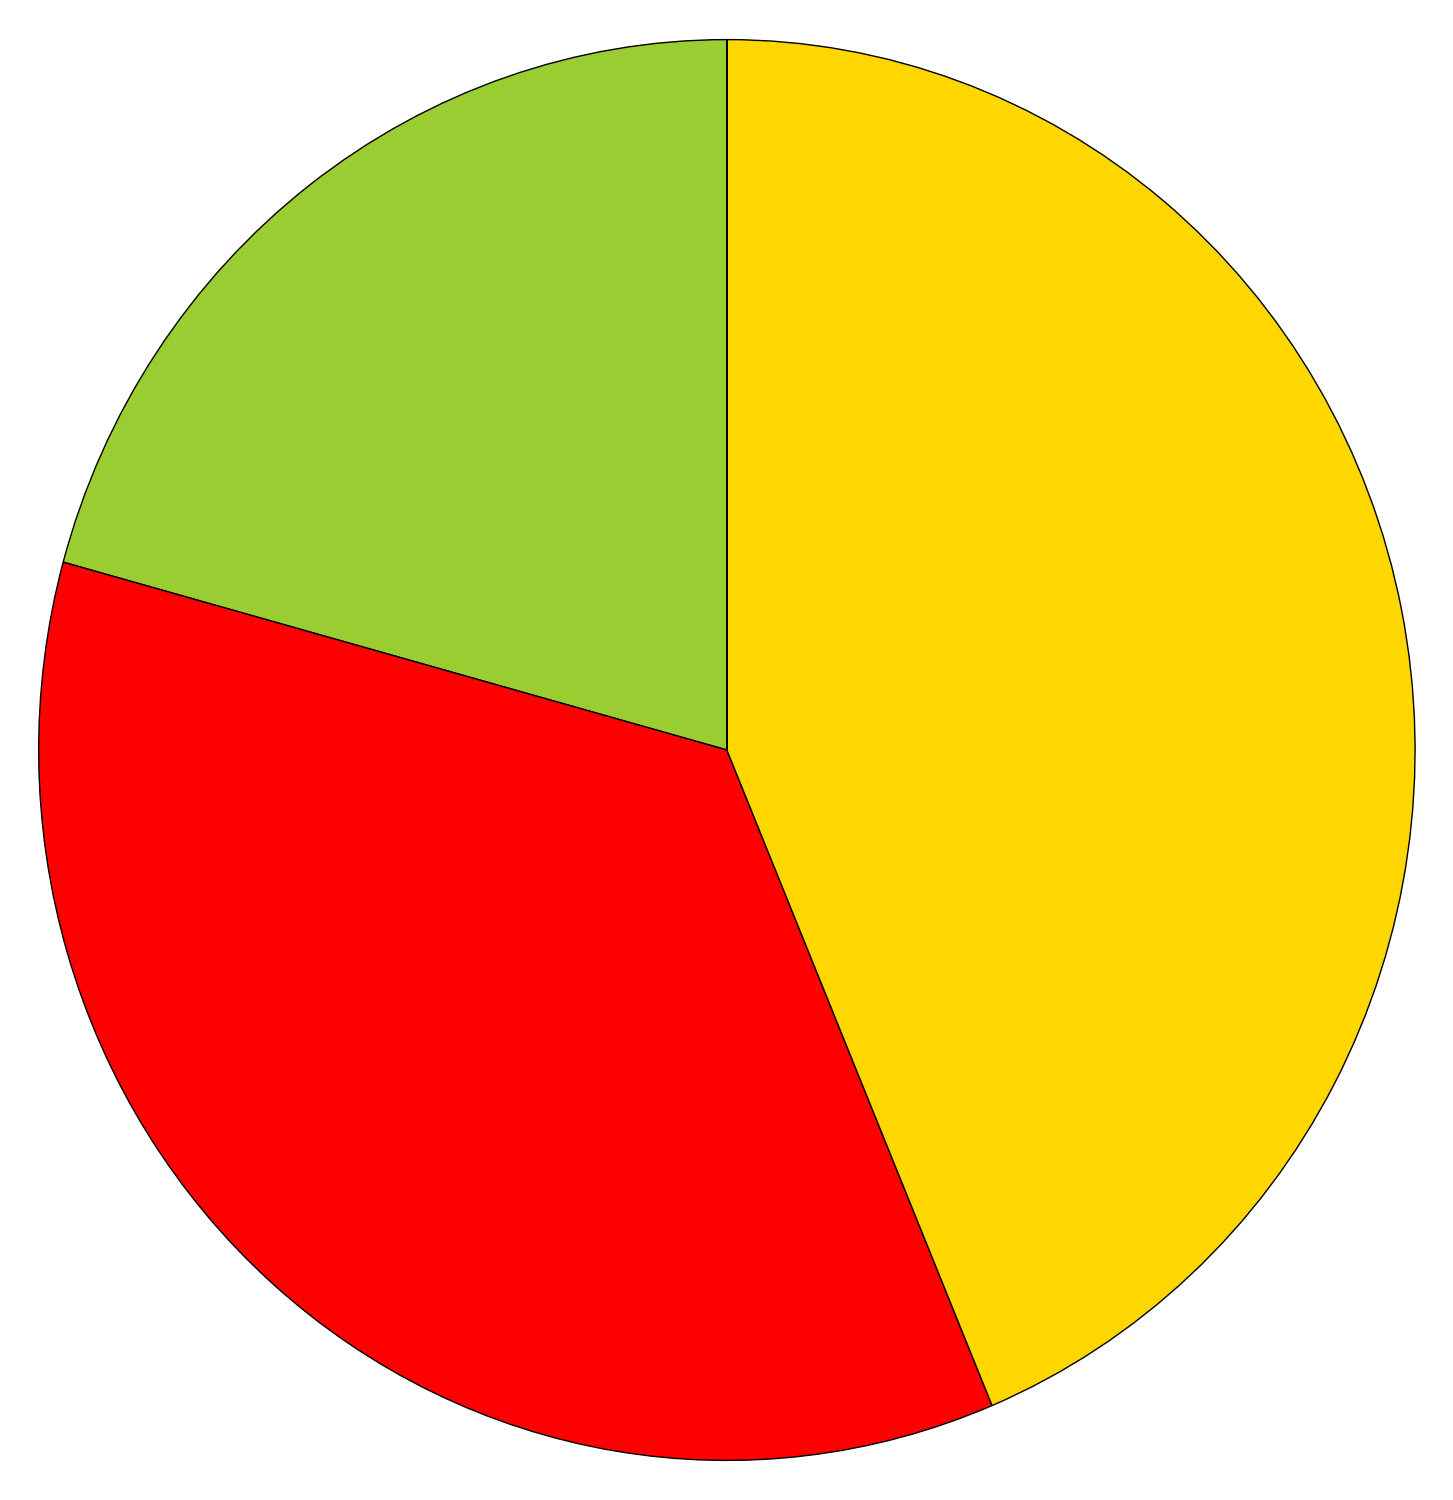
\includegraphics[width=\textwidth]{arousalEEGSVM}
    \caption{SVM}
  \end{subfigure}
  
  \begin{subfigure}[b]{0.3\textwidth}
    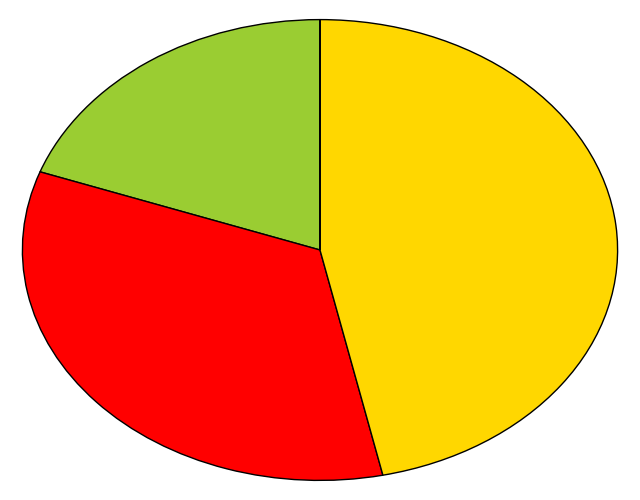
\includegraphics[width=\textwidth]{arousalEEGLDA}
    \caption{LDA}
  \end{subfigure}
  \hfill
  \begin{subfigure}[b]{0.3\textwidth}
    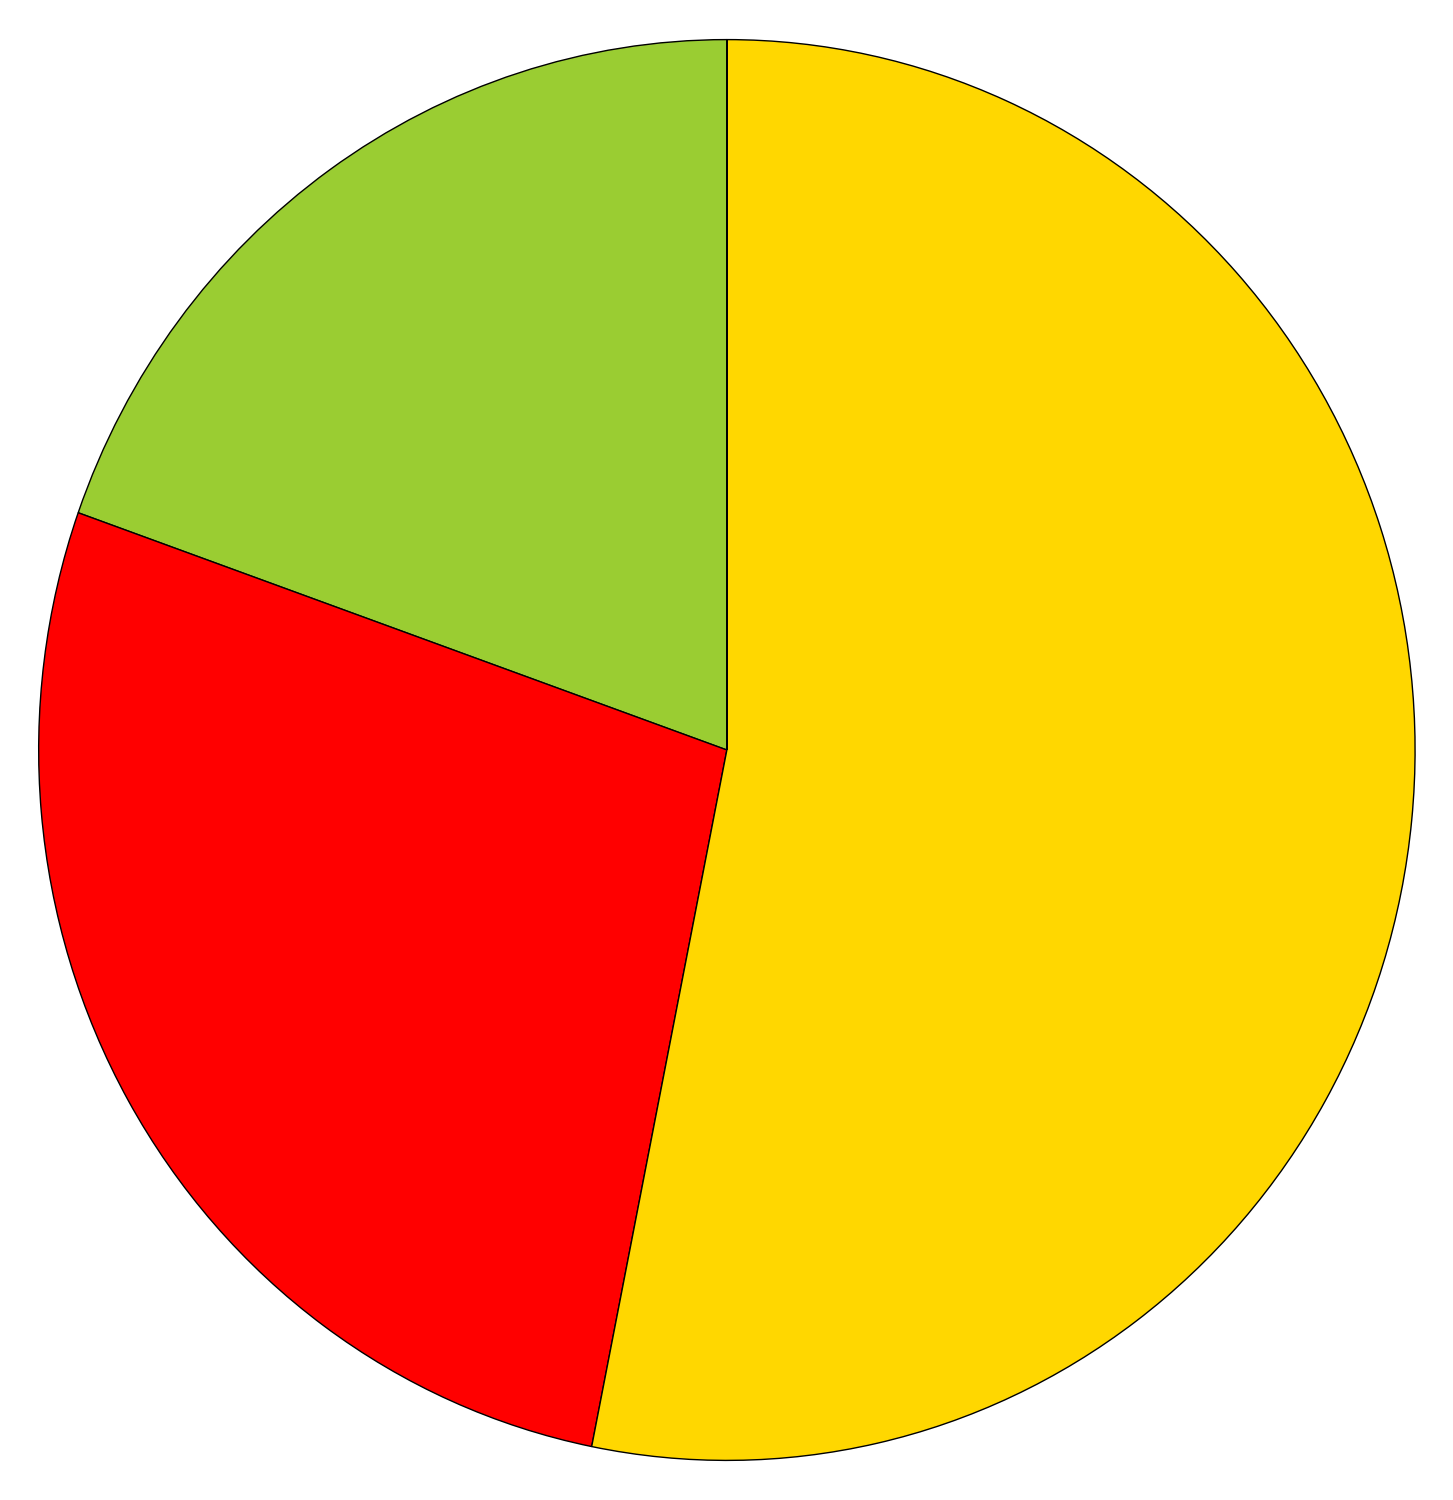
\includegraphics[width=\textwidth]{arousalEEGL1}
    \caption{Lasso regression}
  \end{subfigure}
  \hfill
  \begin{subfigure}[b]{0.3\textwidth}
    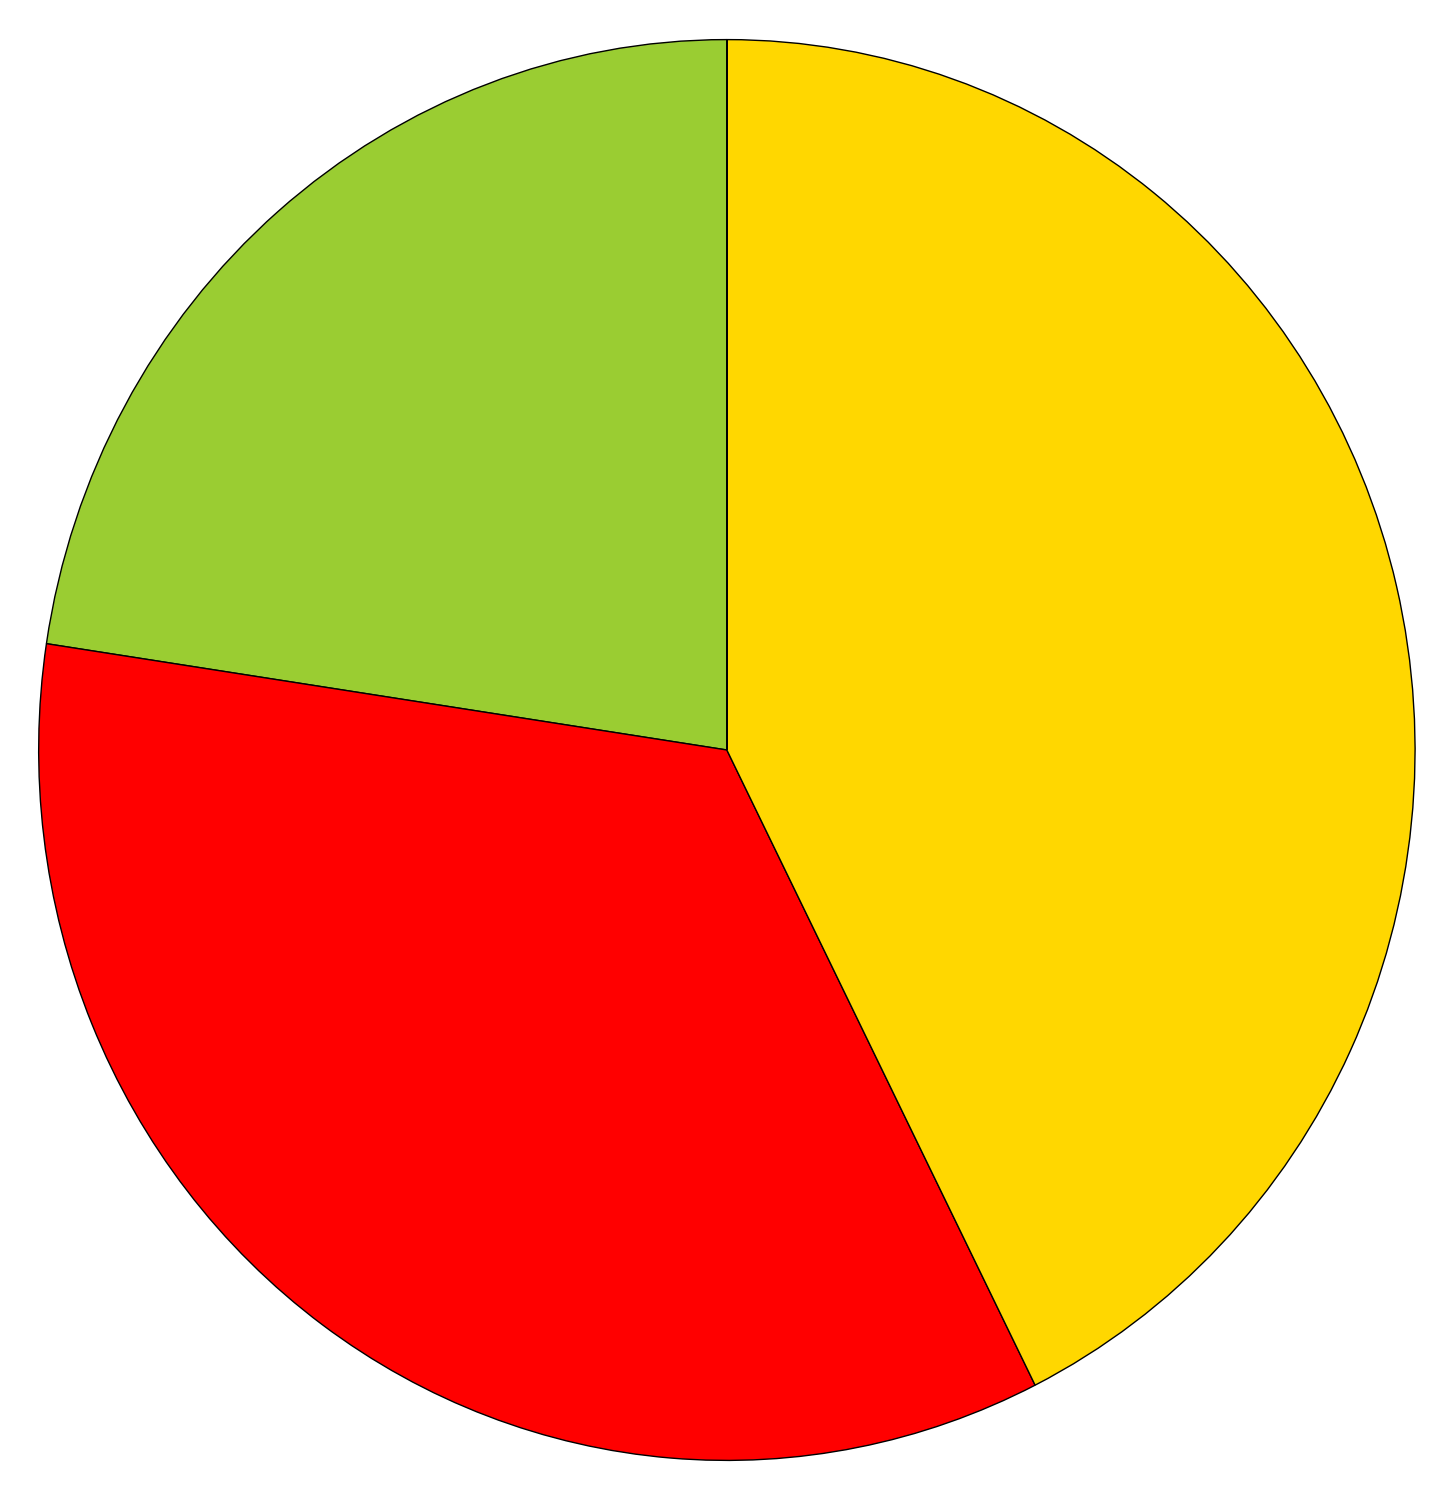
\includegraphics[width=\textwidth]{arousalEEGL2}
    \caption{Ridge regression}
  \end{subfigure}
  
  \begin{subfigure}[b]{0.3\textwidth}
    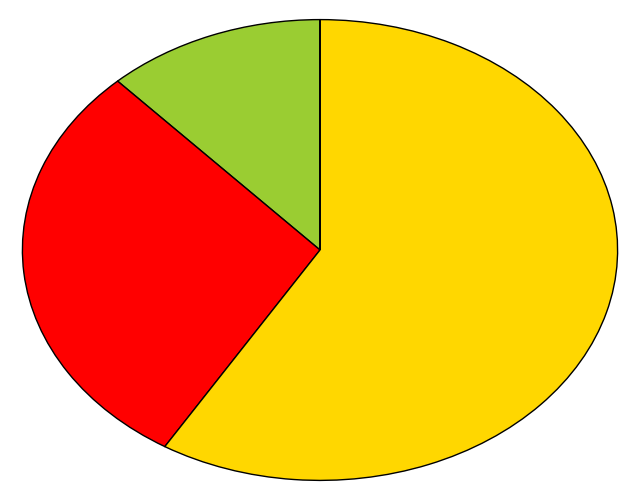
\includegraphics[width=\textwidth]{arousalEEGRF}
    \caption{Random forests}
  \end{subfigure}
  \hfill
  \begin{subfigure}[b]{0.3\textwidth}
    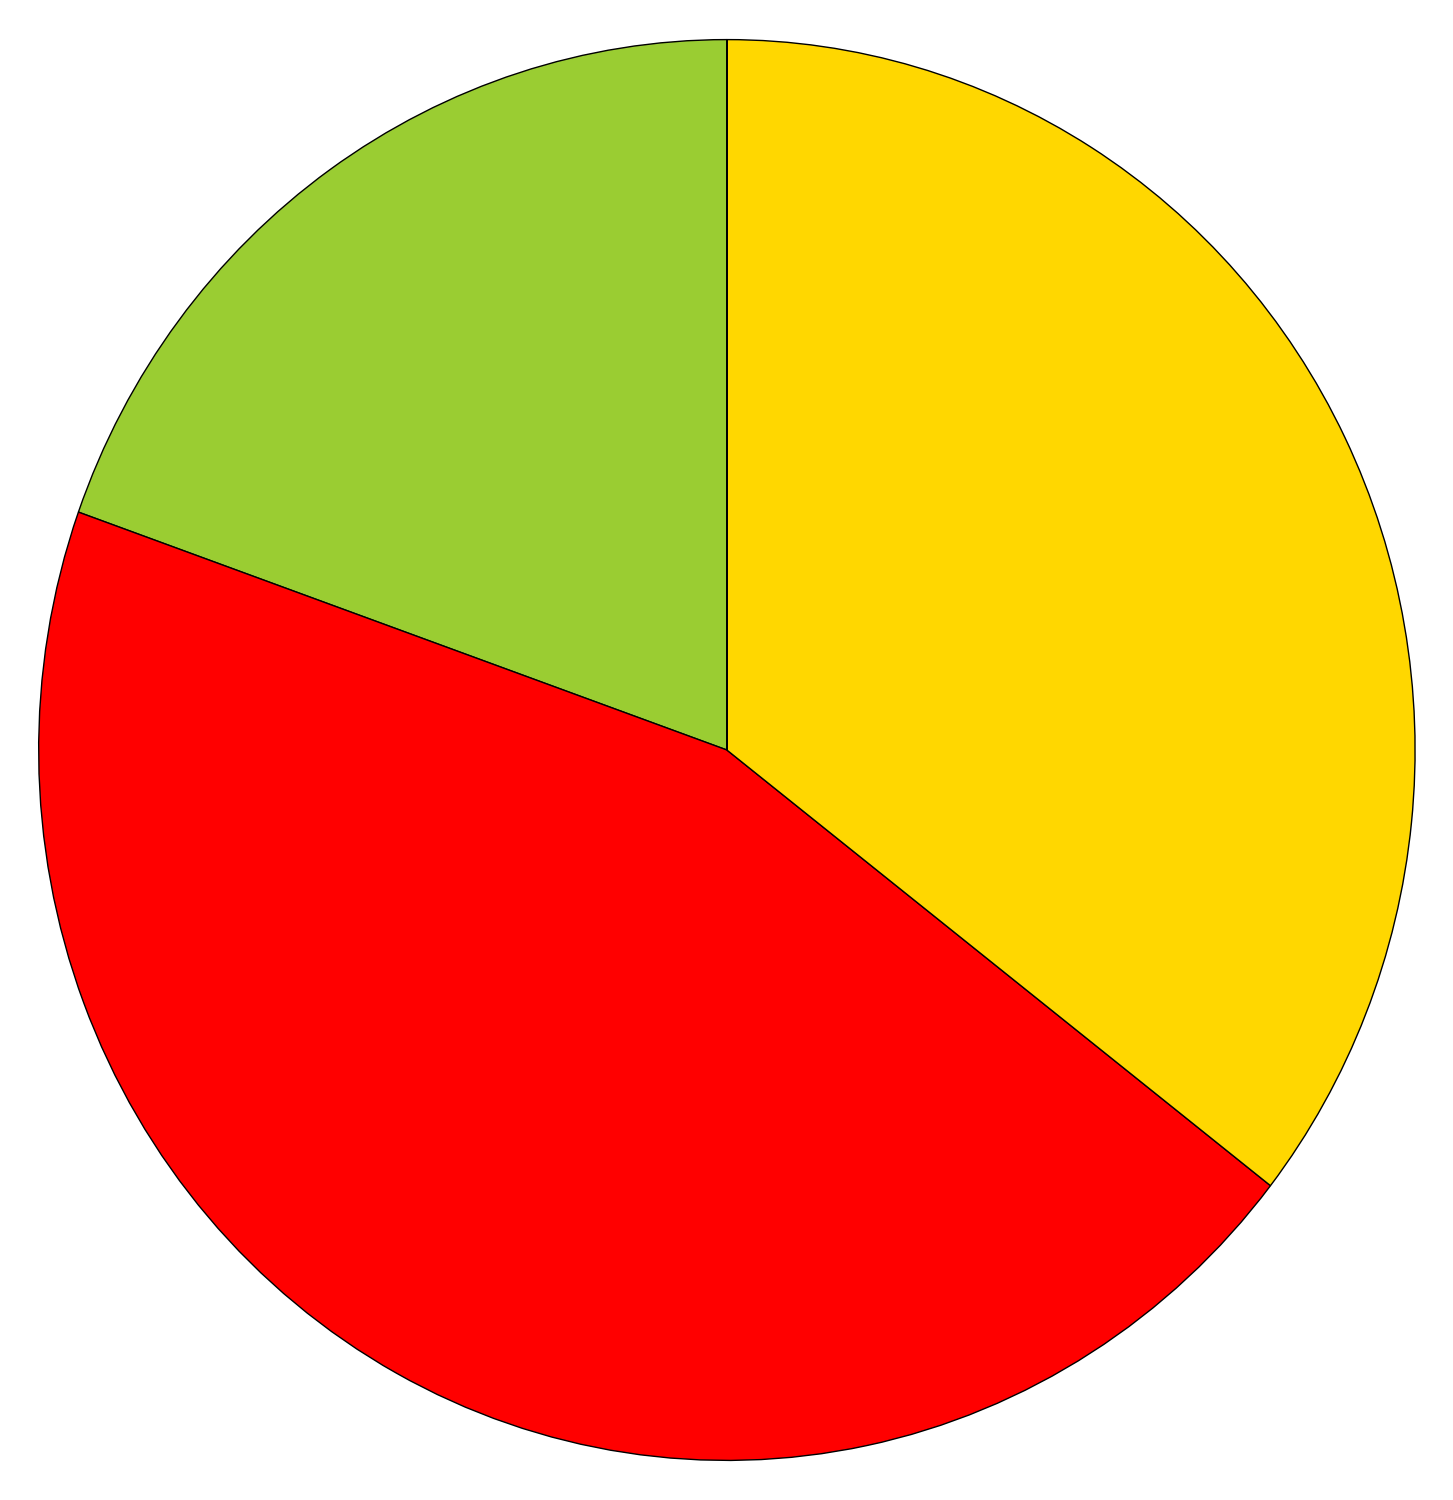
\includegraphics[width=\textwidth]{arousalEEGPCA} %TODO 
    \caption{PCA}
  \end{subfigure}
  \hfill
  \begin{subfigure}[b]{0.3\textwidth}
    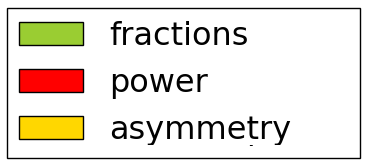
\includegraphics[width=\textwidth]{EEGlegend}
    \caption{Legend\label{arousalpieslegend}}
  \end{subfigure}
\end{figure}

\clearpage

\begin{figure}[!tbp]
  \centering
  \caption{Selection features for valence classification, using only EEG features.\label{valenceEEGpies}}
  \begin{subfigure}[b]{0.3\textwidth}
    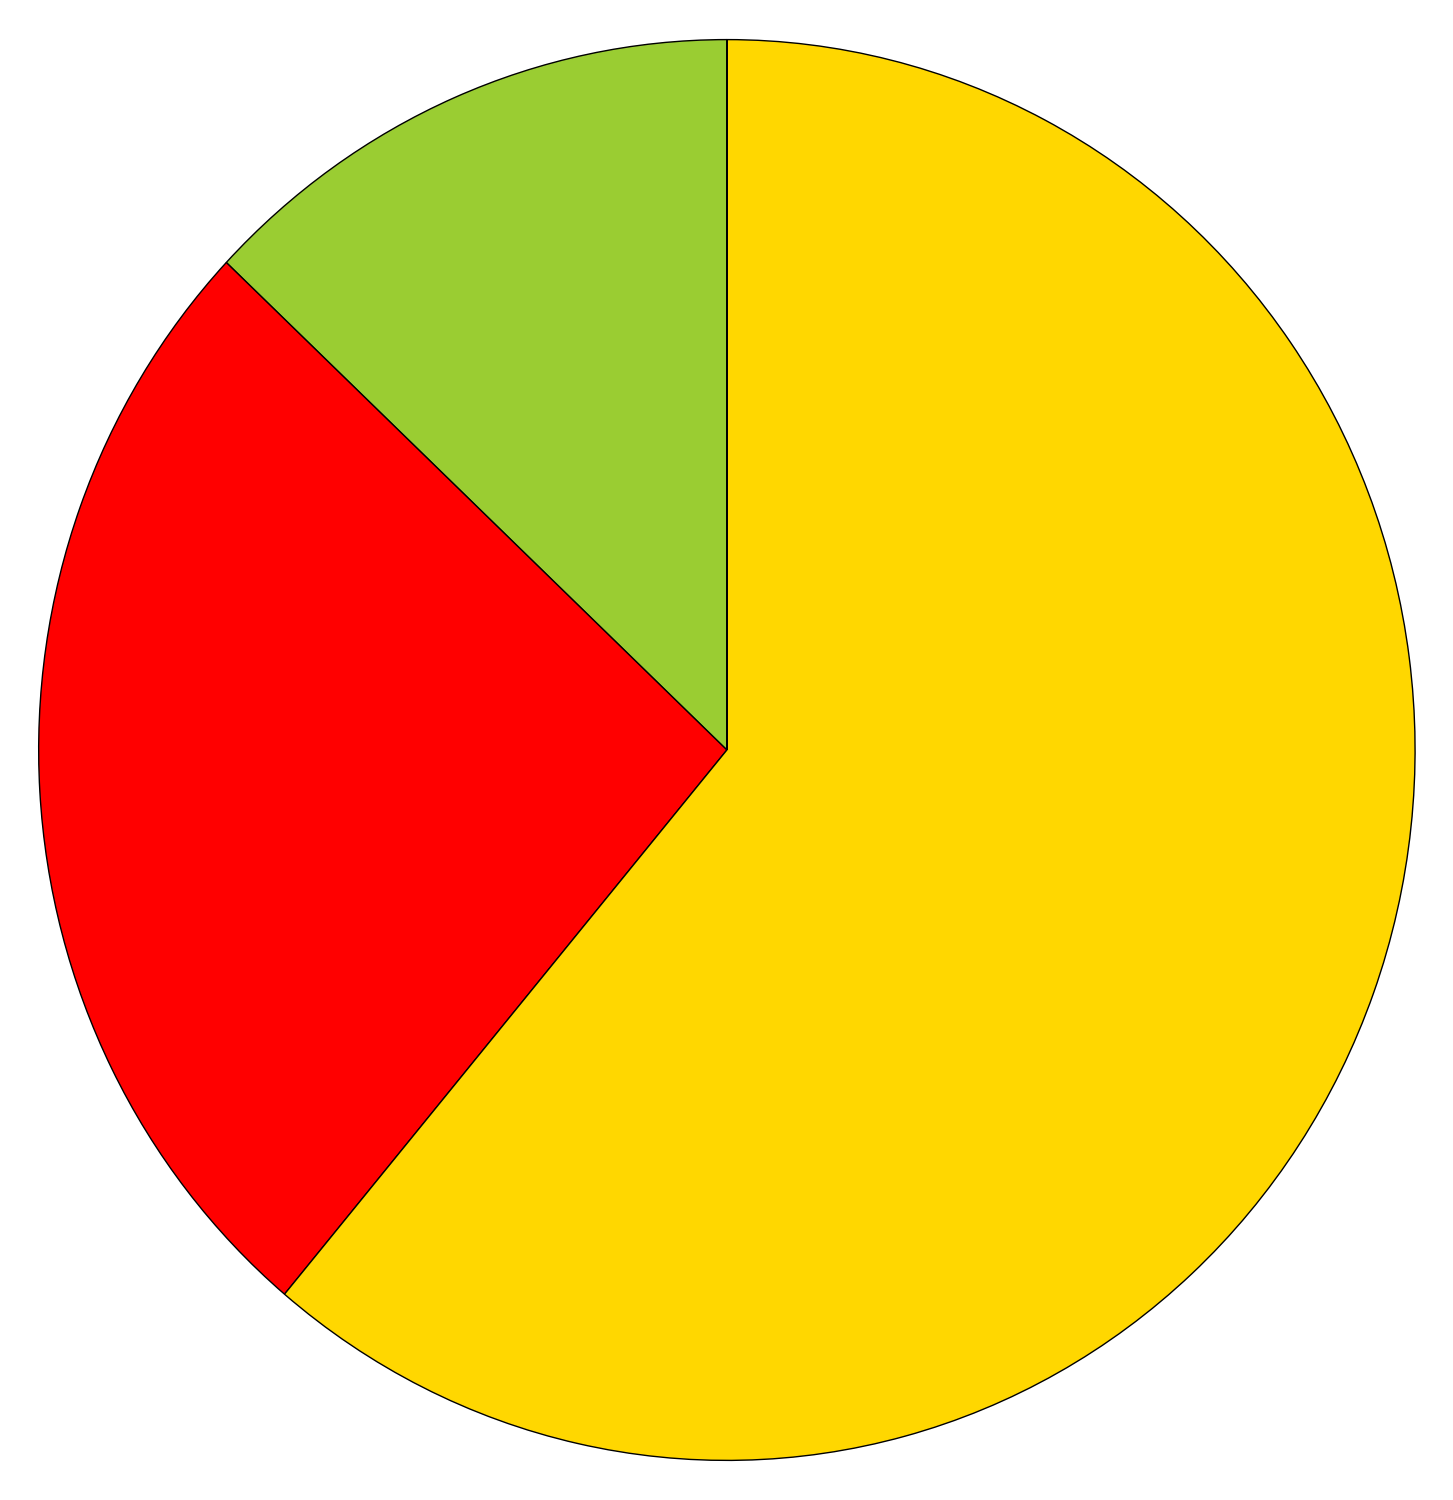
\includegraphics[width=\textwidth]{valenceEEGpearsonR}
    \caption{Pearson correlation}
  \end{subfigure}
  \hfill
  \begin{subfigure}[b]{0.3\textwidth}
    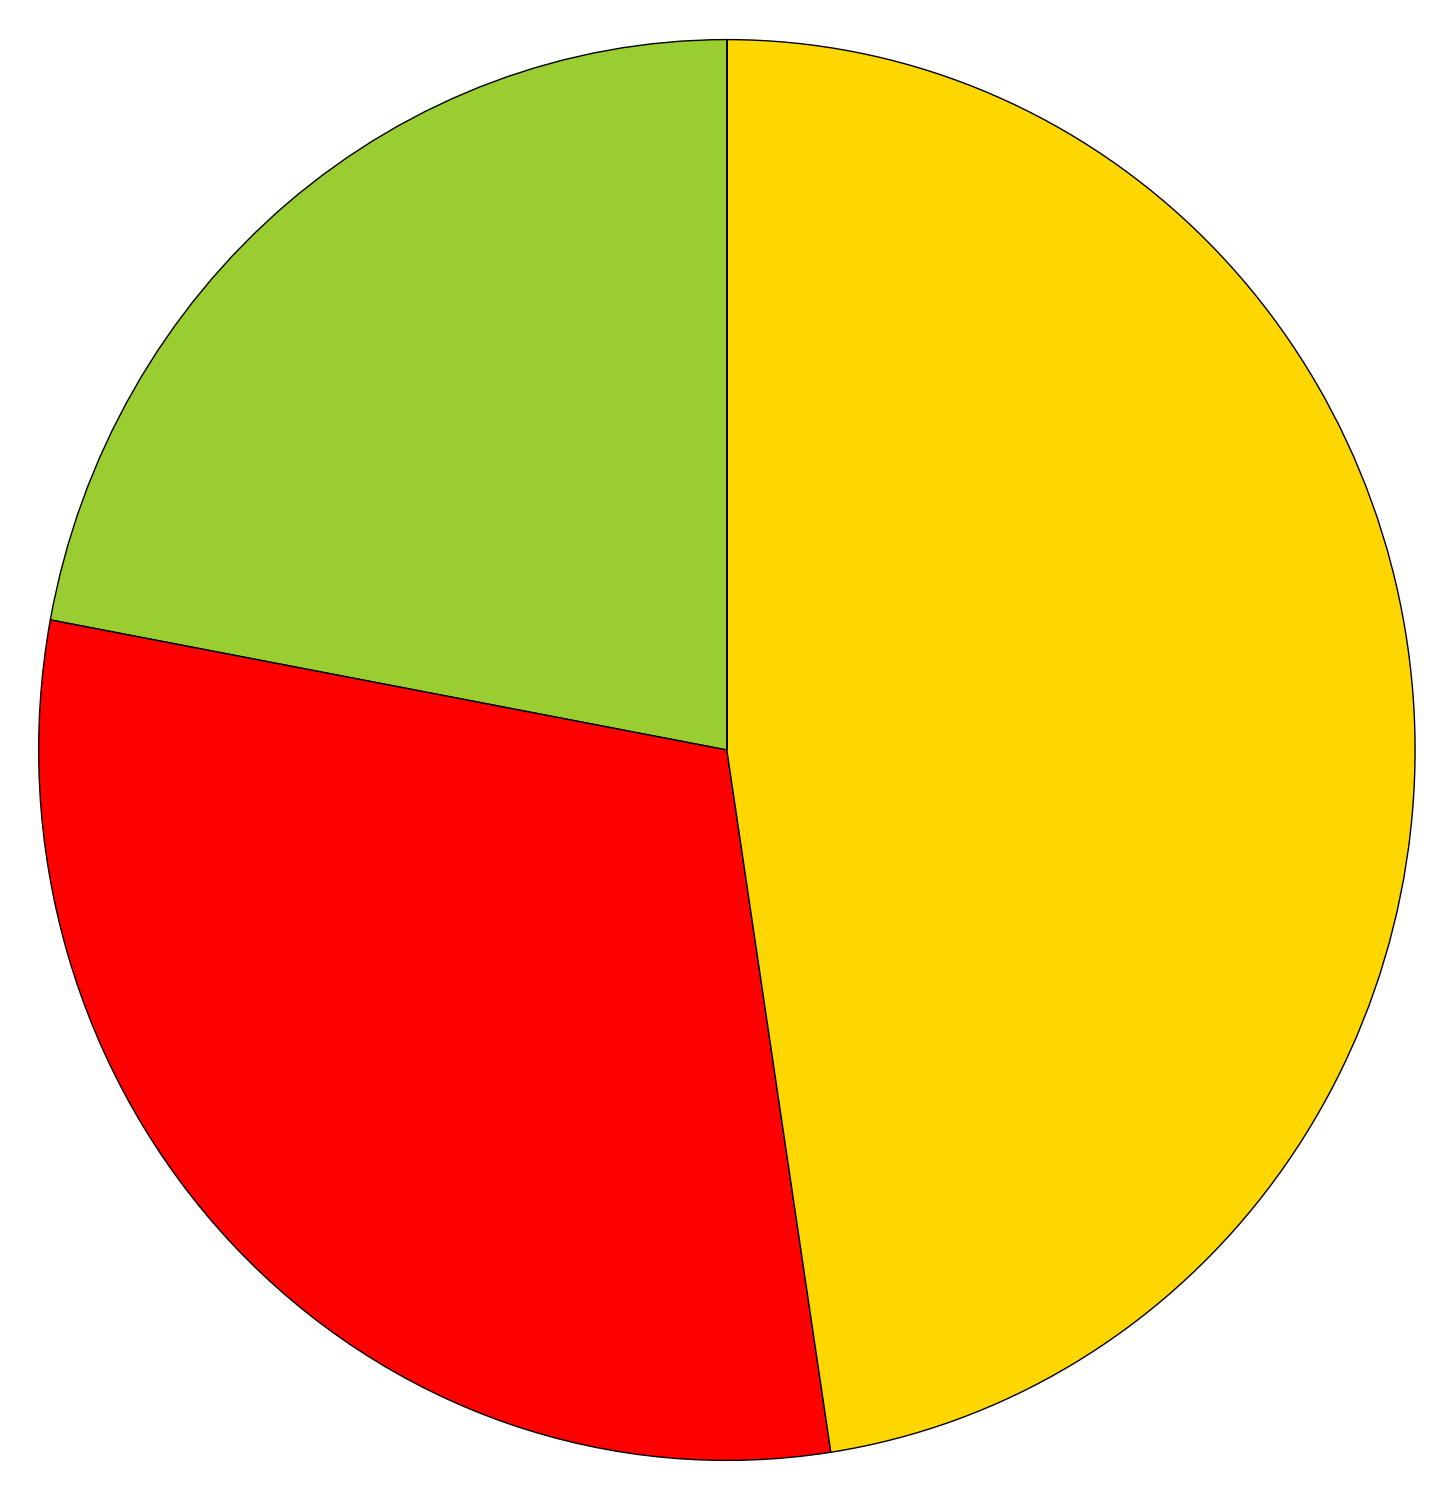
\includegraphics[width=\textwidth]{valenceEEGMutInf}
    \caption{Mutual information}
  \end{subfigure}
  \hfill
  \begin{subfigure}[b]{0.3\textwidth}
    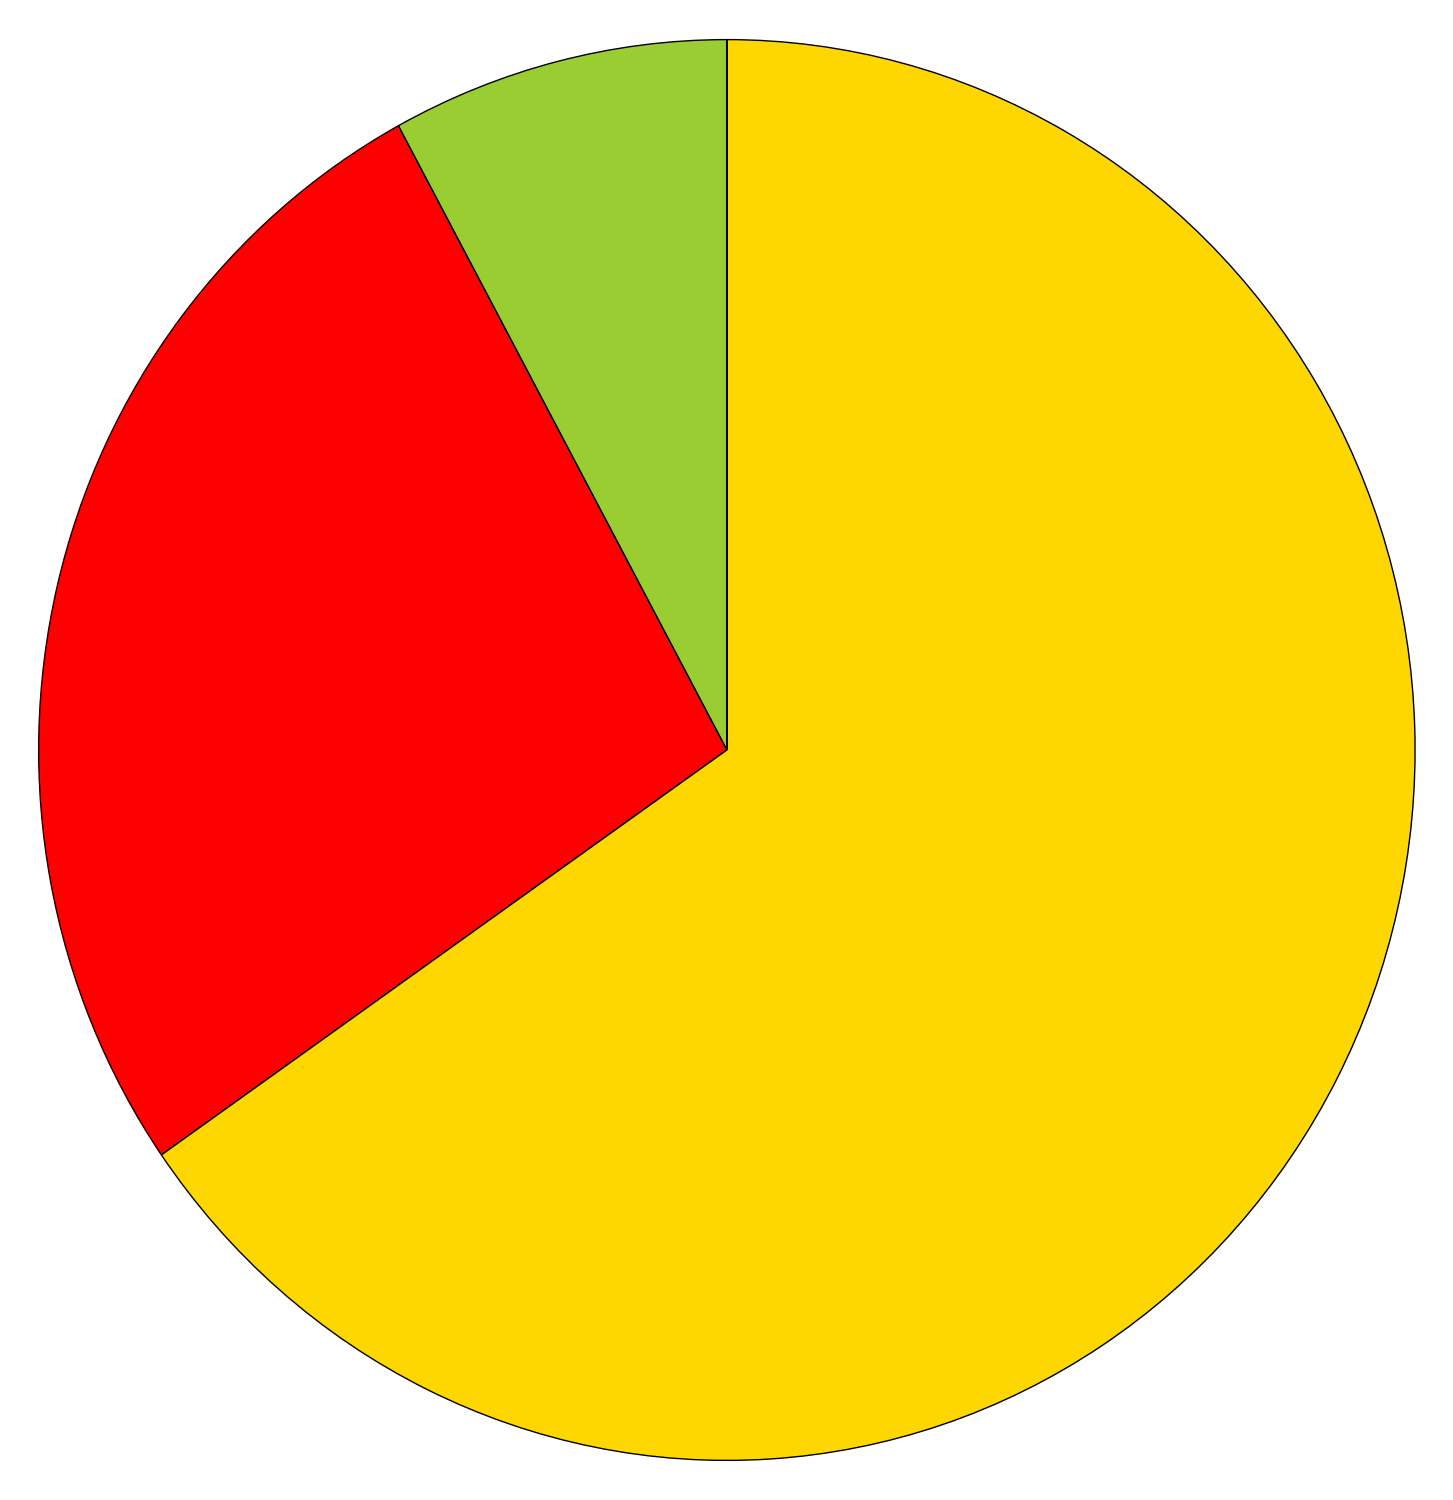
\includegraphics[width=\textwidth]{valenceEEGdCorr}
    \caption{Distance Correlation}
  \end{subfigure}
  
  \begin{subfigure}[b]{0.3\textwidth}
    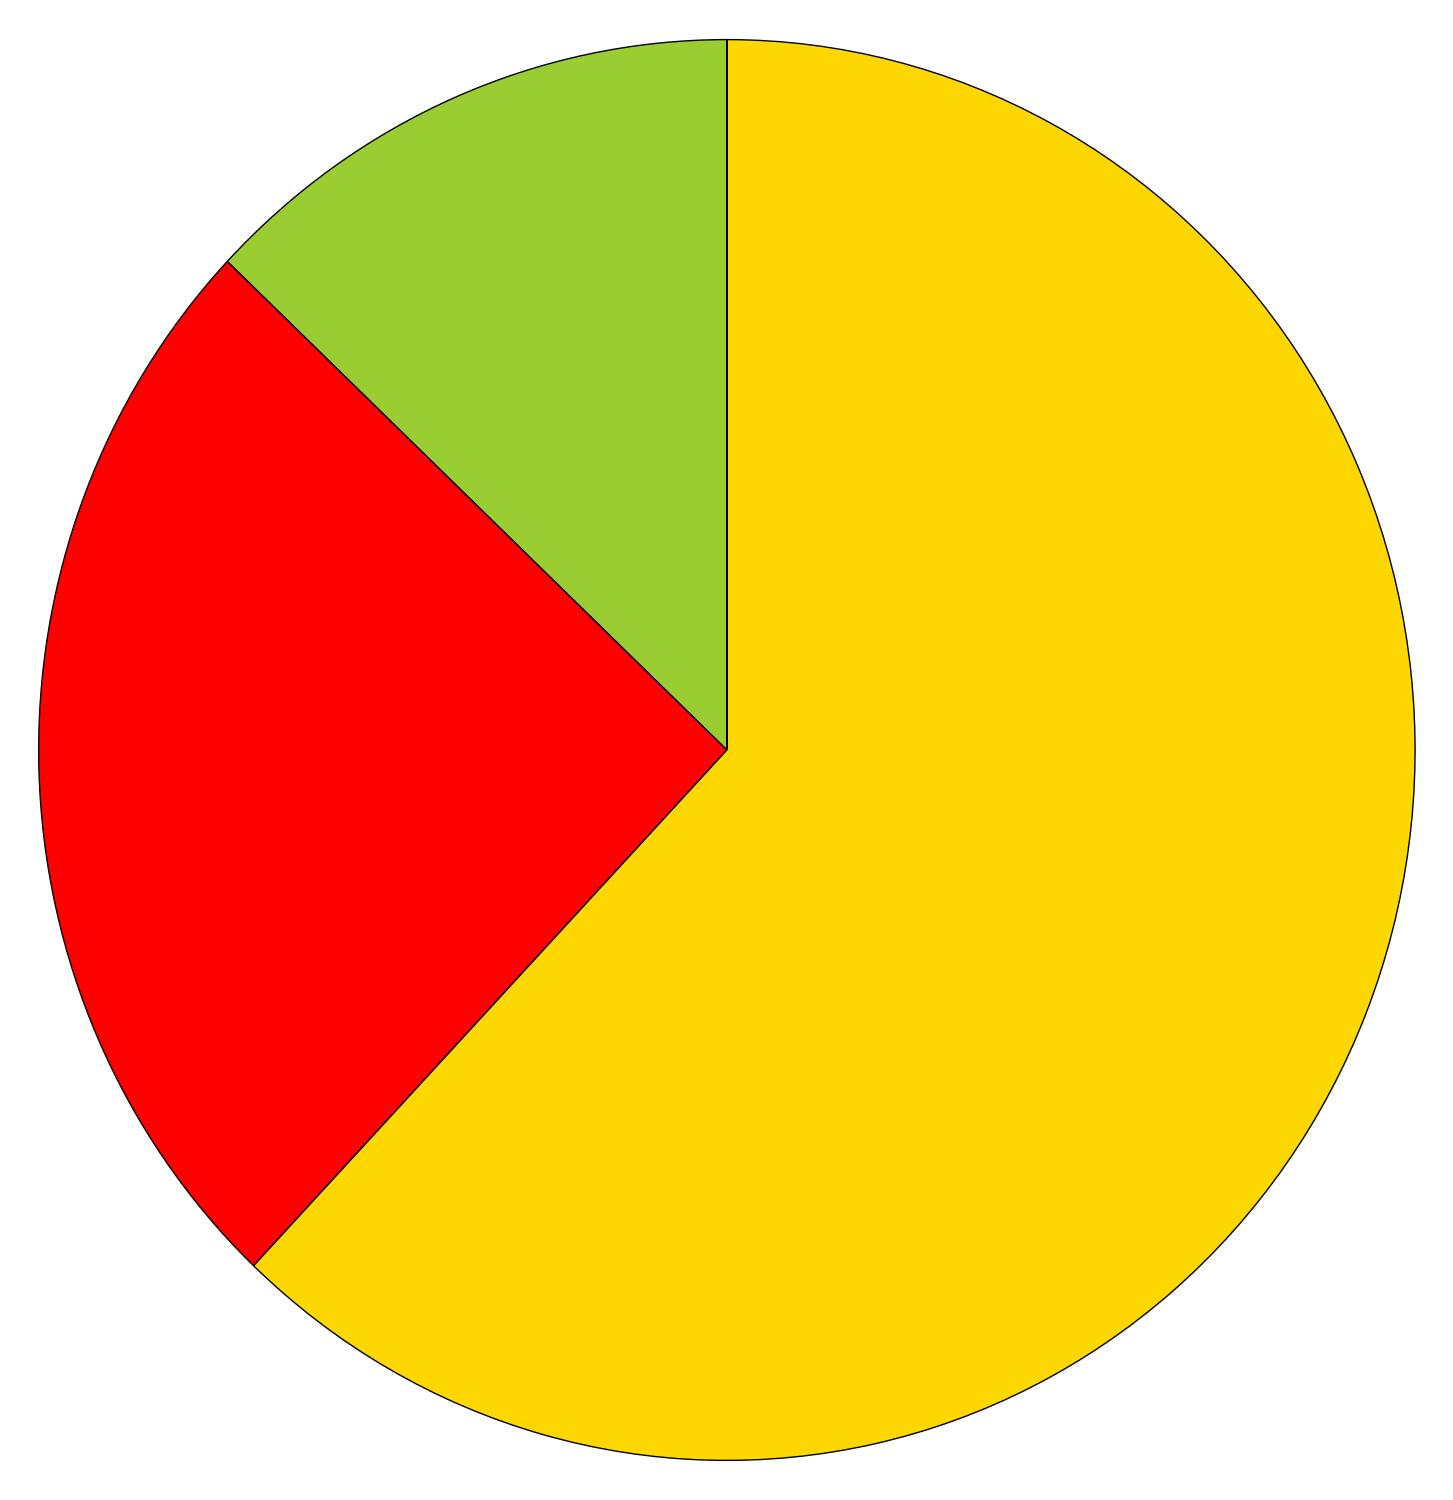
\includegraphics[width=\textwidth]{valenceEEGANOVA}
    \caption{ANOVA}
  \end{subfigure}
  \hfill
  \begin{subfigure}[b]{0.3\textwidth}
    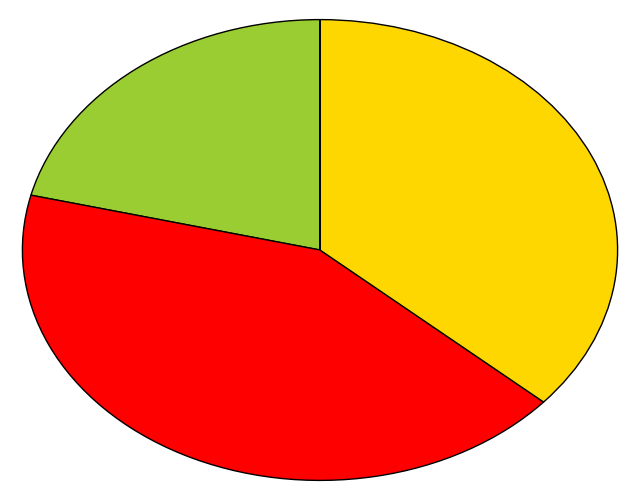
\includegraphics[width=\textwidth]{valenceEEGLR}
    \caption{Linear regression}
  \end{subfigure}
  \hfill
  \begin{subfigure}[b]{0.3\textwidth}
    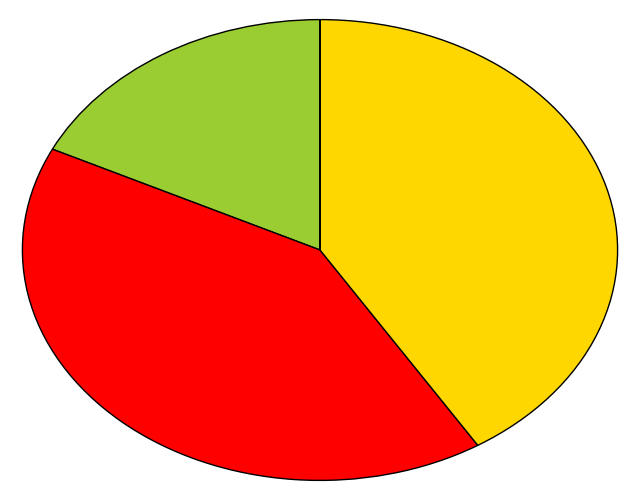
\includegraphics[width=\textwidth]{valenceEEGSVM}
    \caption{SVM}
  \end{subfigure}
  
  \begin{subfigure}[b]{0.3\textwidth}
    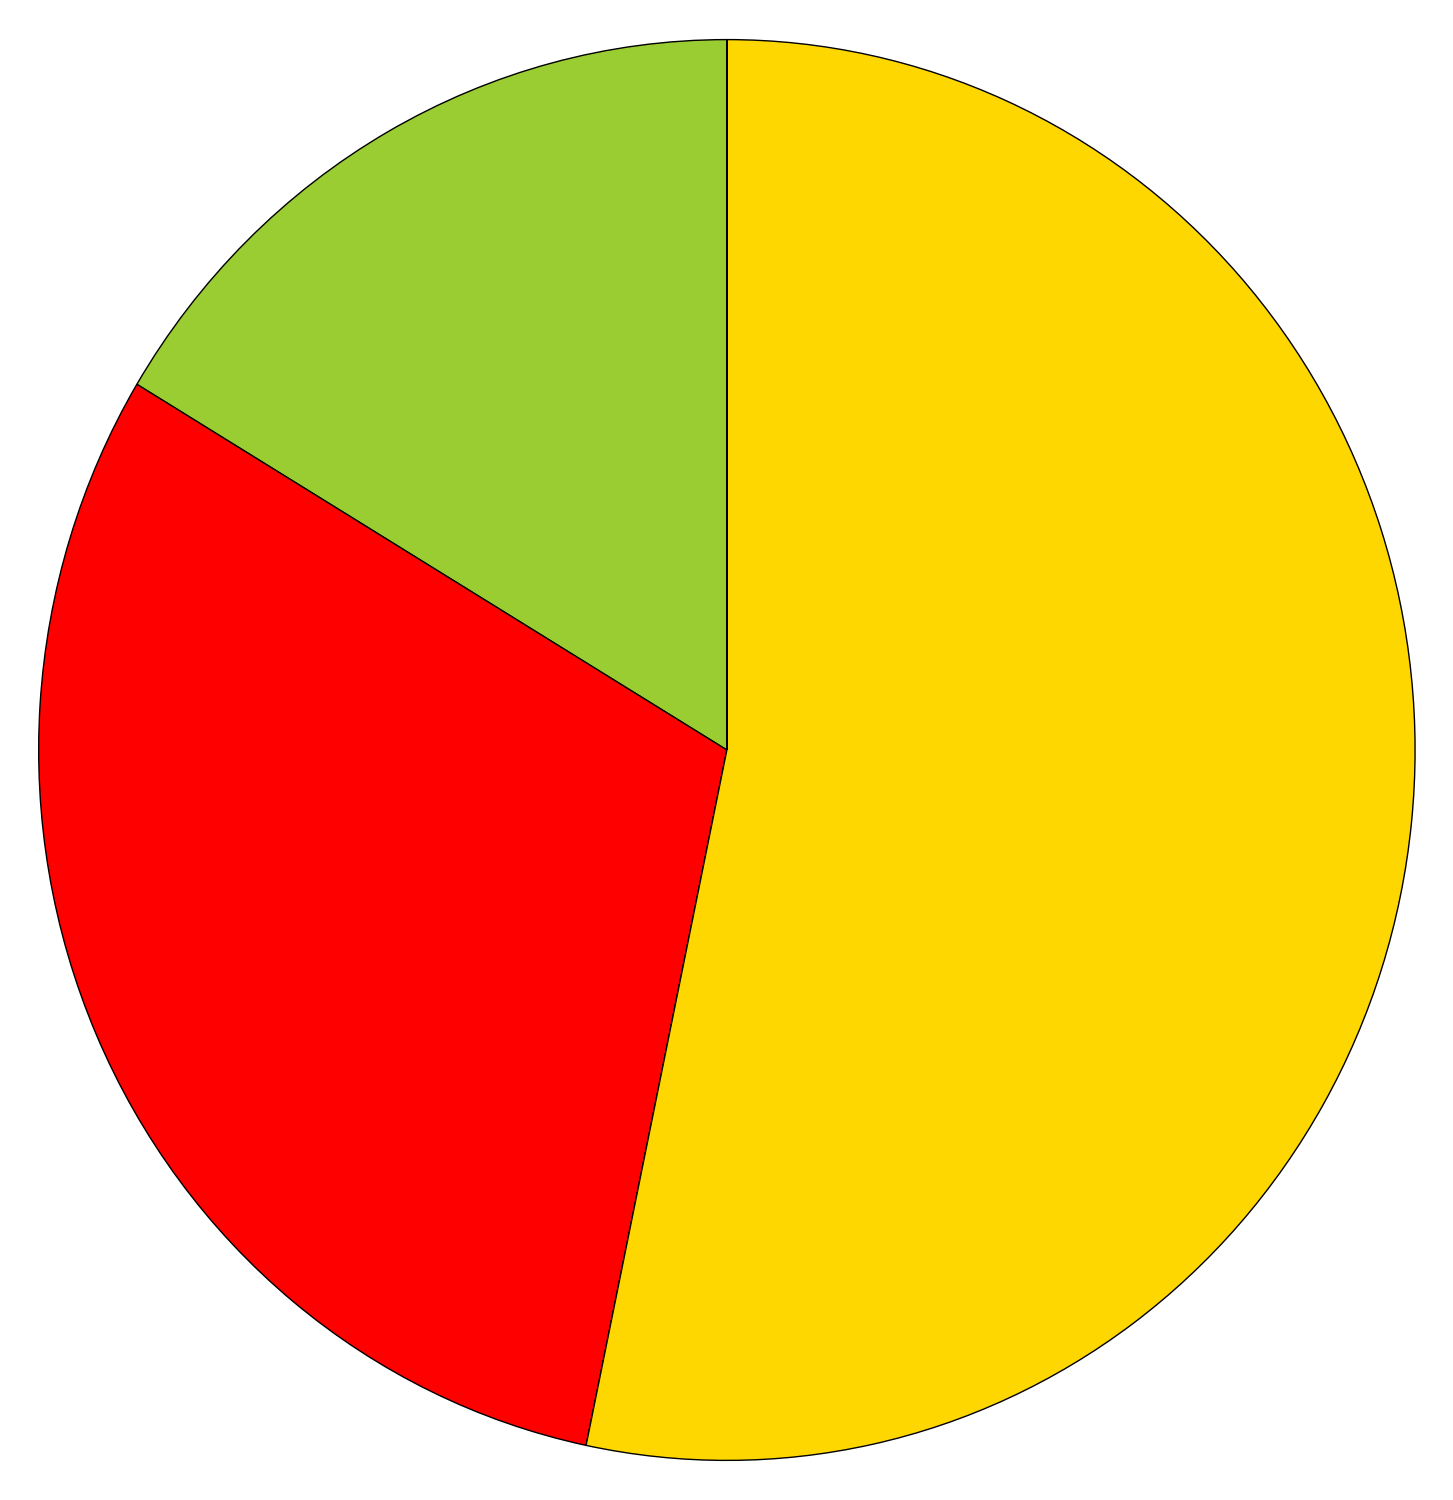
\includegraphics[width=\textwidth]{valenceEEGLDA}
    \caption{LDA}
  \end{subfigure}
  \hfill
  \begin{subfigure}[b]{0.3\textwidth}
    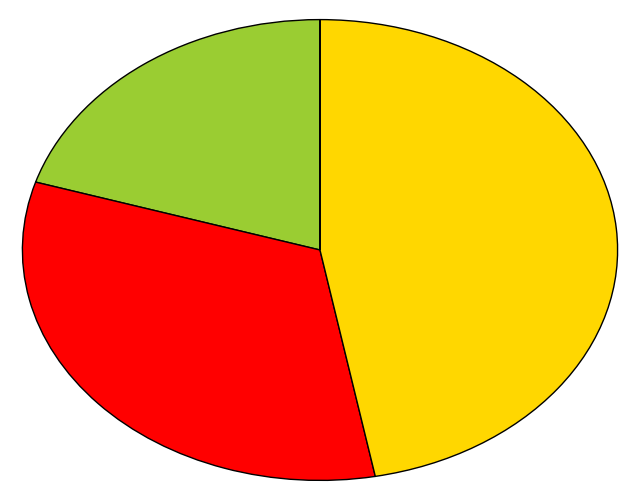
\includegraphics[width=\textwidth]{valenceEEGL1}
    \caption{Lasso regression}
  \end{subfigure}
  \hfill
  \begin{subfigure}[b]{0.3\textwidth}
    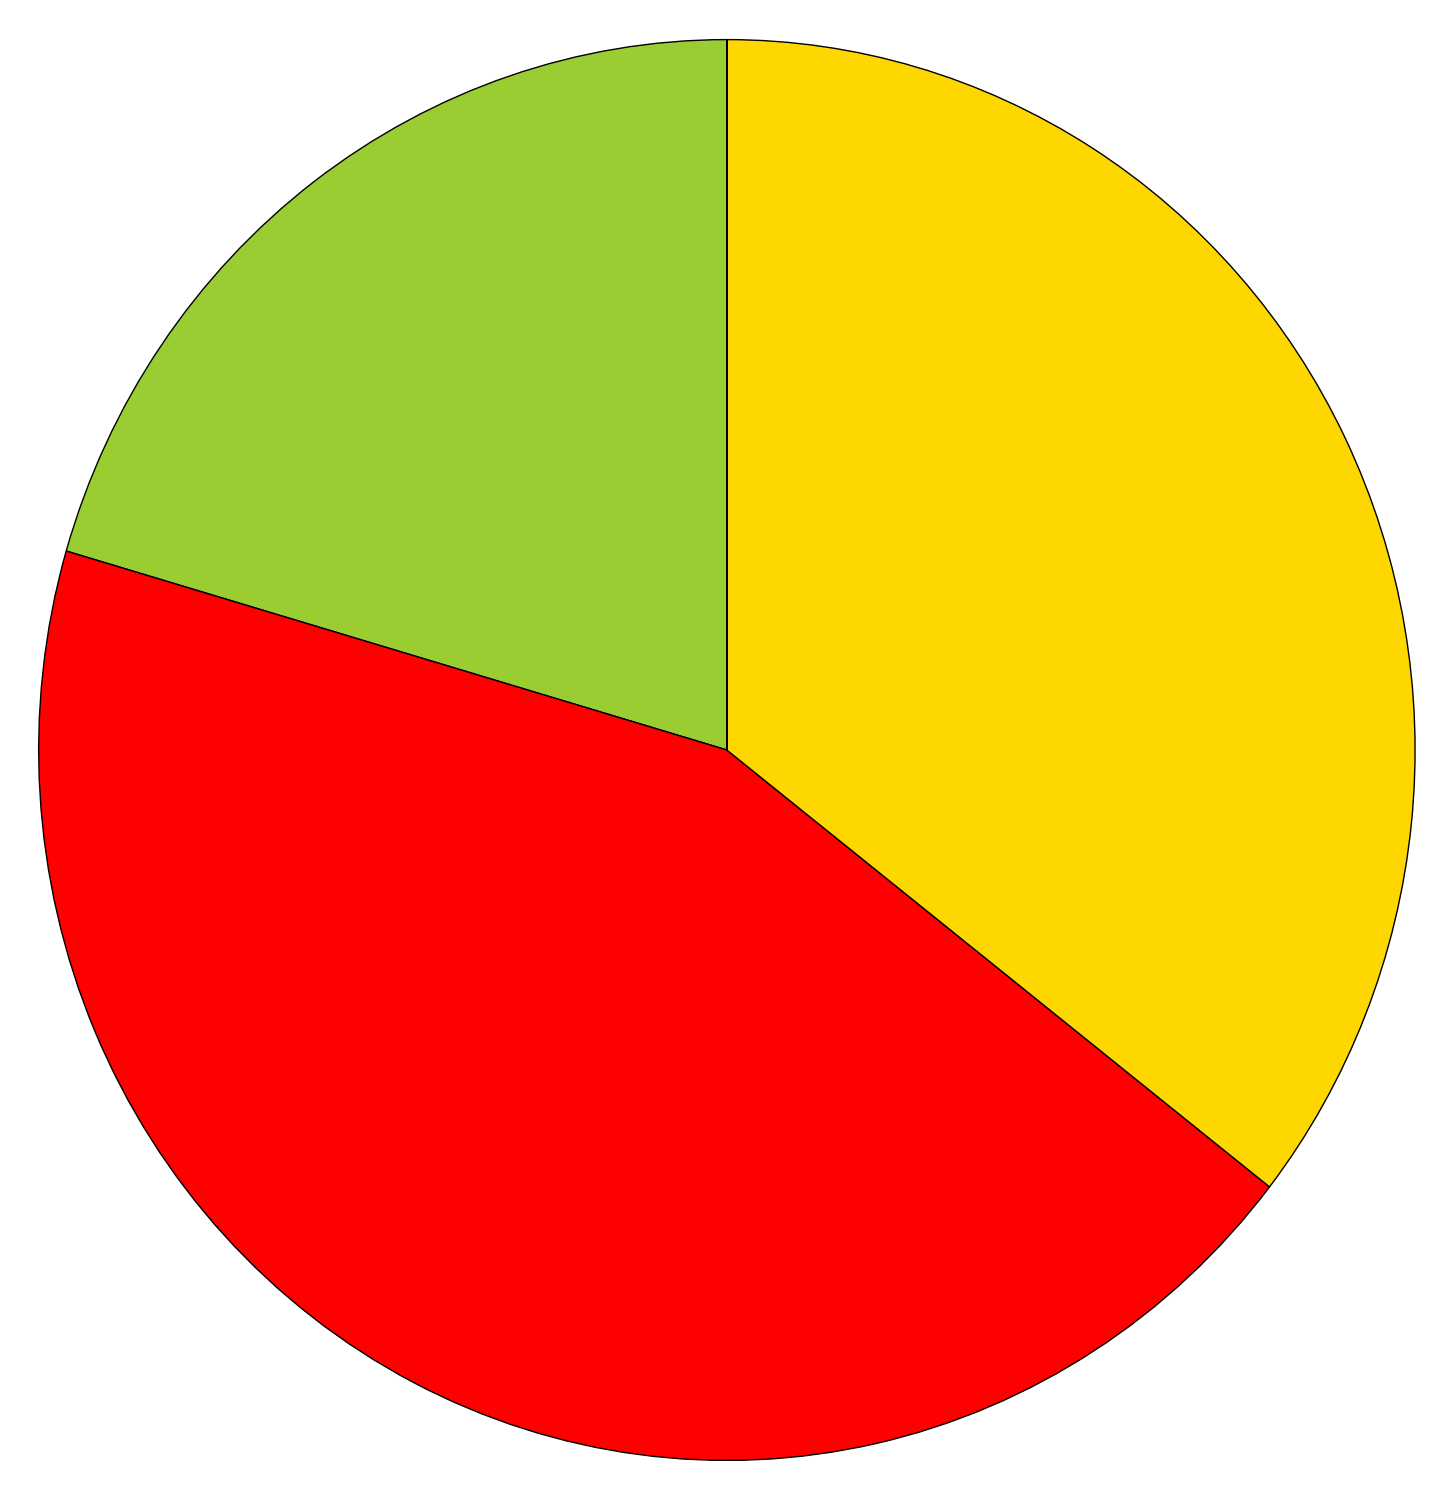
\includegraphics[width=\textwidth]{valenceEEGL2}
    \caption{Ridge regression}
  \end{subfigure}
  
  \begin{subfigure}[b]{0.3\textwidth}
    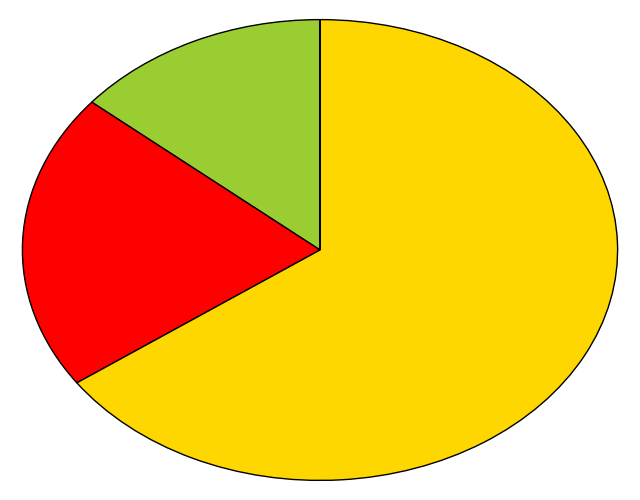
\includegraphics[width=\textwidth]{valenceEEGRF}
    \caption{Random forests}
  \end{subfigure}
  \hfill
  \begin{subfigure}[b]{0.3\textwidth}
    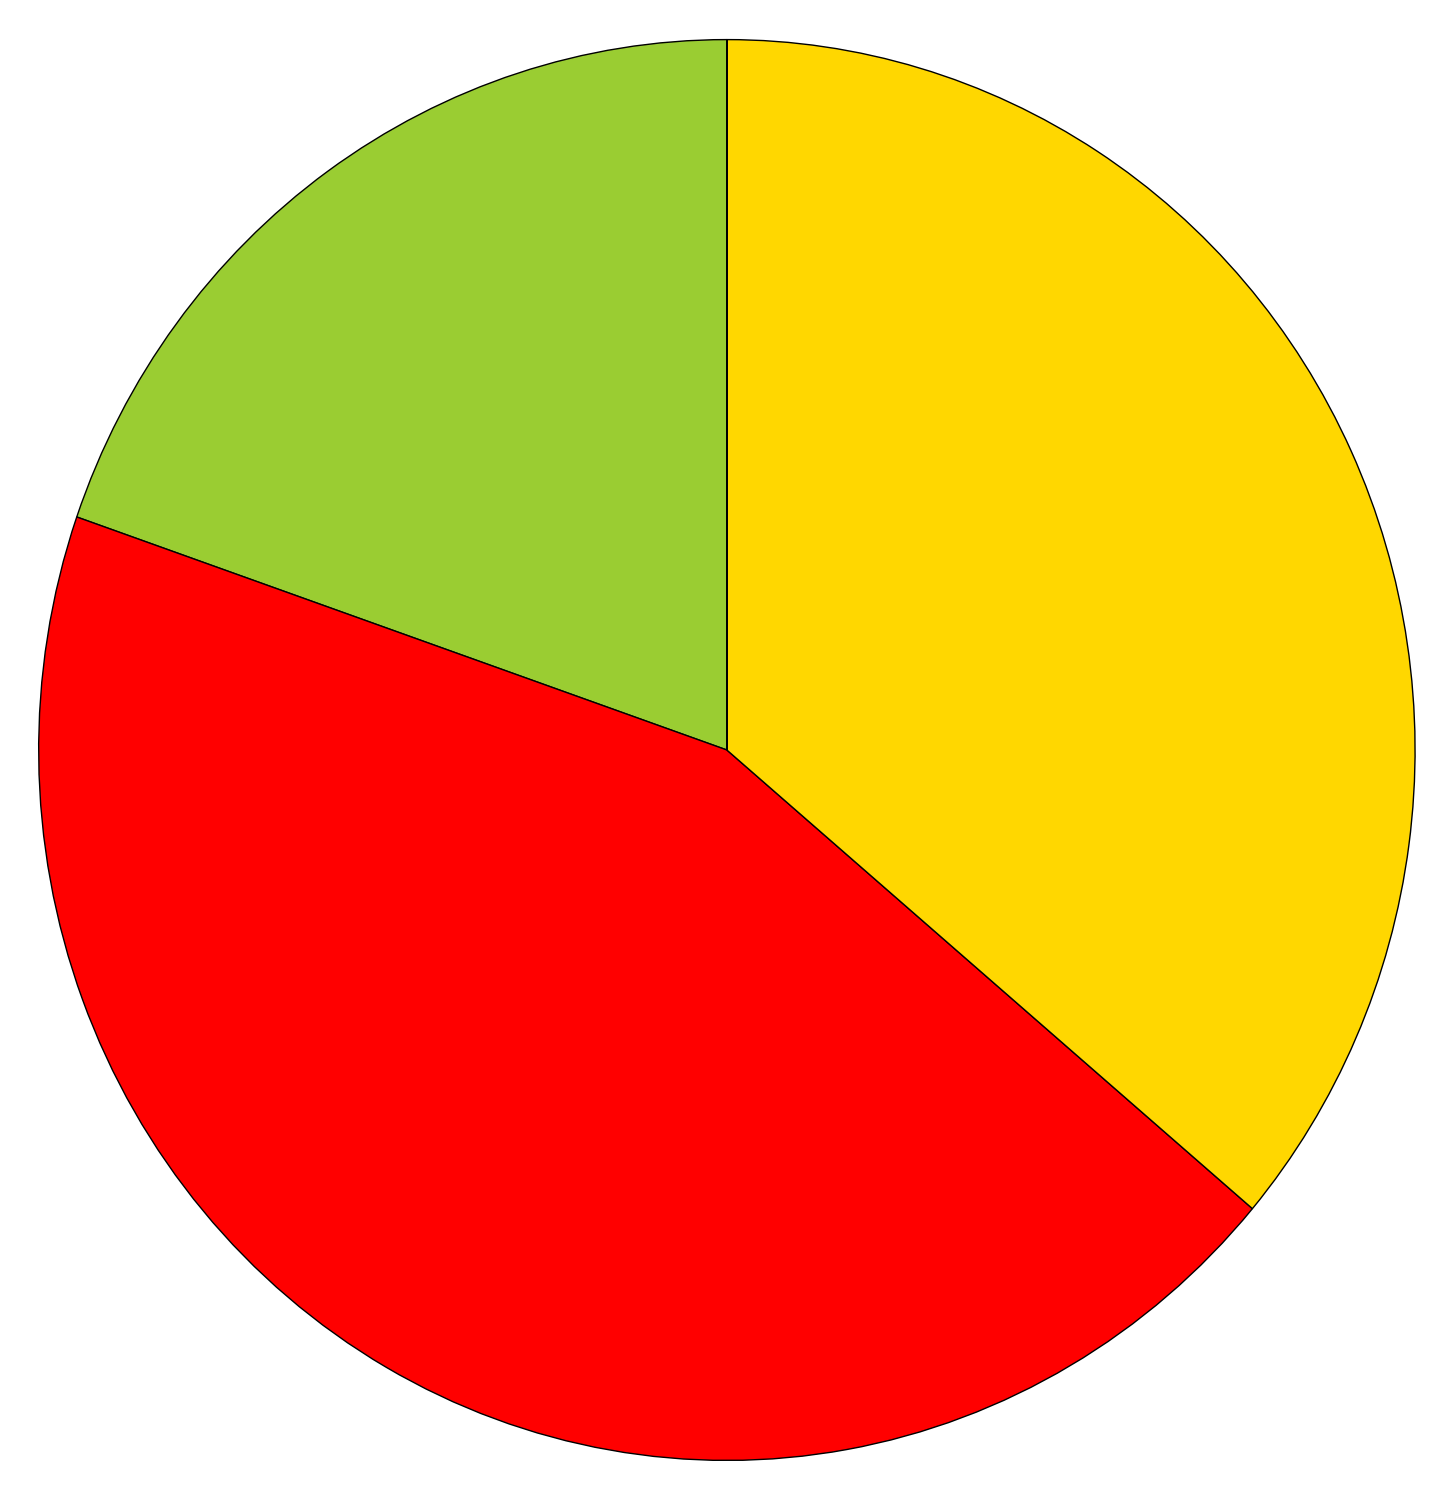
\includegraphics[width=\textwidth]{valenceEEGPCA} %TODO 
    \caption{PCA}
  \end{subfigure}
  \hfill
  \begin{subfigure}[b]{0.3\textwidth}
    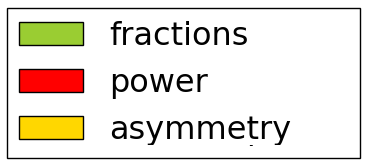
\includegraphics[width=\textwidth]{EEGlegend}
    \caption{Legend\label{valencepieslegend}}
  \end{subfigure}
\end{figure}
\clearpage
%regions
%TODO

\clearpage
\begin{figure}[!tbp]
  \centering
  \caption{Selection features for arousal classification, using only non-EEG features.\label{arousalnon-EEGpies}}
  \begin{subfigure}[b]{0.3\textwidth}
    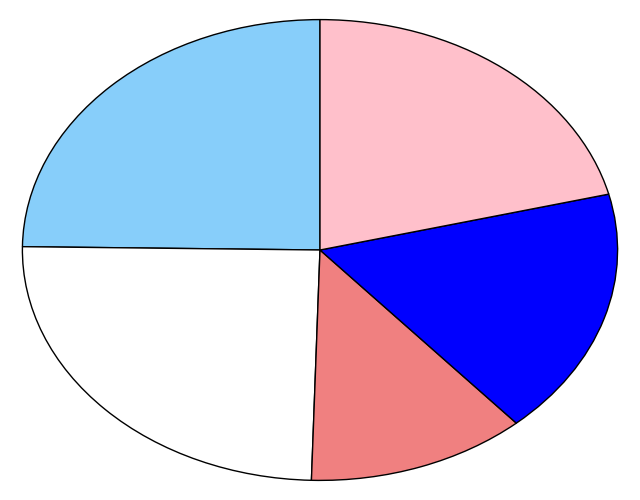
\includegraphics[width=\textwidth]{arousalnon-EEGpearsonR}
    \caption{Pearson correlation}
  \end{subfigure}
  \hfill
  \begin{subfigure}[b]{0.3\textwidth}
    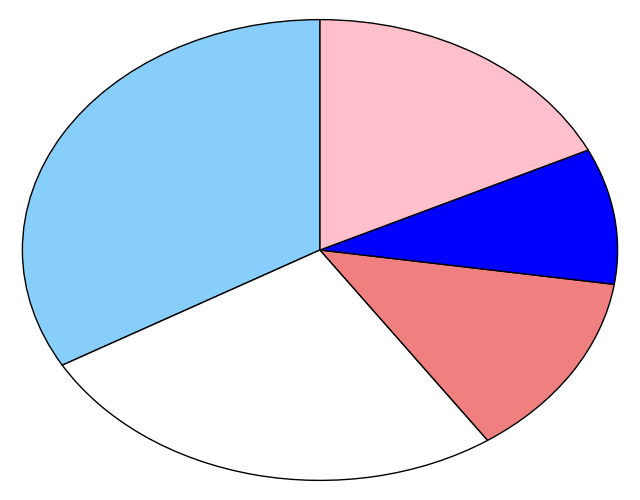
\includegraphics[width=\textwidth]{arousalnon-EEGMutInf}
    \caption{Mutual information}
  \end{subfigure}
  \hfill
  \begin{subfigure}[b]{0.3\textwidth}
    \includegraphics[width=\textwidth]{arousalnon-EEGdCorr}
    \caption{Distance Correlation}
  \end{subfigure}
  
  \begin{subfigure}[b]{0.3\textwidth}
    \includegraphics[width=\textwidth]{arousalnon-EEGANOVA}
    \caption{ANOVA}
  \end{subfigure}
  \hfill
  \begin{subfigure}[b]{0.3\textwidth}
    \includegraphics[width=\textwidth]{arousalnon-EEGLR}
    \caption{Linear regression}
  \end{subfigure}
  \hfill
  \begin{subfigure}[b]{0.3\textwidth}
    \includegraphics[width=\textwidth]{arousalnon-EEGSVM}
    \caption{SVM}
  \end{subfigure}
  
  \begin{subfigure}[b]{0.3\textwidth}
    \includegraphics[width=\textwidth]{arousalnon-EEGLDA}
    \caption{LDA}
  \end{subfigure}
  \hfill
  \begin{subfigure}[b]{0.3\textwidth}
    \includegraphics[width=\textwidth]{arousalnon-EEGL1}
    \caption{Lasso regression}
  \end{subfigure}
  \hfill
  \begin{subfigure}[b]{0.3\textwidth}
    \includegraphics[width=\textwidth]{arousalnon-EEGL2}
    \caption{Ridge regression}
  \end{subfigure}
  
  \begin{subfigure}[b]{0.3\textwidth}
    \includegraphics[width=\textwidth]{arousalnon-EEGRF}
    \caption{Random forests}
  \end{subfigure}
  \hfill
  \begin{subfigure}[b]{0.3\textwidth}
    \includegraphics[width=\textwidth]{arousalnon-EEGPCA} %TODO 
    \caption{PCA}
  \end{subfigure}
  \hfill
  \begin{subfigure}[b]{0.3\textwidth}
    \includegraphics[width=\textwidth]{non-EEGlegend}
    \caption{Legend\label{arousalpieslegend}}
  \end{subfigure}
\end{figure}

\clearpage

\begin{figure}[!tbp]
  \centering
  \caption{Selection features for valence classification, using only non-EEG features.\label{valencenon-EEGpies}}
  \begin{subfigure}[b]{0.3\textwidth}
    \includegraphics[width=\textwidth]{valencenon-EEGpearsonR}
    \caption{Pearson correlation}
  \end{subfigure}
  \hfill
  \begin{subfigure}[b]{0.3\textwidth}
    \includegraphics[width=\textwidth]{valencenon-EEGMutInf}
    \caption{Mutual information}
  \end{subfigure}
  \hfill
  \begin{subfigure}[b]{0.3\textwidth}
    \includegraphics[width=\textwidth]{valencenon-EEGdCorr}
    \caption{Distance Correlation}
  \end{subfigure}
  
  \begin{subfigure}[b]{0.3\textwidth}
    \includegraphics[width=\textwidth]{valencenon-EEGANOVA}
    \caption{ANOVA}
  \end{subfigure}
  \hfill
  \begin{subfigure}[b]{0.3\textwidth}
    \includegraphics[width=\textwidth]{valencenon-EEGLR}
    \caption{Linear regression}
  \end{subfigure}
  \hfill
  \begin{subfigure}[b]{0.3\textwidth}
    \includegraphics[width=\textwidth]{valencenon-EEGSVM}
    \caption{SVM}
  \end{subfigure}
  
  \begin{subfigure}[b]{0.3\textwidth}
    \includegraphics[width=\textwidth]{valencenon-EEGLDA}
    \caption{LDA}
  \end{subfigure}
  \hfill
  \begin{subfigure}[b]{0.3\textwidth}
    \includegraphics[width=\textwidth]{valencenon-EEGL1}
    \caption{Lasso regression}
  \end{subfigure}
  \hfill
  \begin{subfigure}[b]{0.3\textwidth}
    \includegraphics[width=\textwidth]{valencenon-EEGL2}
    \caption{Ridge regression}
  \end{subfigure}
  
  \begin{subfigure}[b]{0.3\textwidth}
    \includegraphics[width=\textwidth]{valencenon-EEGRF}
    \caption{Random forests}
  \end{subfigure}
  \hfill
  \begin{subfigure}[b]{0.3\textwidth}
    \includegraphics[width=\textwidth]{valencenon-EEGPCA} %TODO 
    \caption{PCA}
  \end{subfigure}
  \hfill
  \begin{subfigure}[b]{0.3\textwidth}
    \includegraphics[width=\textwidth]{non-EEGlegend}
    \caption{Legend\label{valencepieslegend}}
  \end{subfigure}
\end{figure}
\clearpage
